\documentclass{article}
\usepackage{../homework-problems-UMB}

\toggletrue{solutions}
\toggletrue{answers}
%\togglefalse{solutions}

\renewcommand{\course}{Math 242}
\renewcommand{\Arccos}{\arccos}
\renewcommand{\Arcsin}{\arcsin}
\renewcommand{\Arctan}{\arctan}
\renewcommand{\Arccot}{{\text{arccot }}}


%\begin{comment}
\homeworkStart{on Lecture 1 \\Quiz date to be announced in class}{}
\item Find the distance between the points. The answer key has not been proofread, use with caution.
\begin{enumerate}
\item $(2, 3, 5)$ and $(3, 5, 7)$.
\answer{$3$}
\item $(1, 1, 1)$ and $(0, 0, -1)$.
\answer{$\sqrt{6}$}
\item A vertex of a cube with edge 2cm and the midpoint of one of the three opposing sides.
\answer{$\sqrt{6}$}
\item Consider a cube with edge 2cm. Consider two edges that do not have a common point and are not parallel. Find the distance between the midpoints of those two edges. 
\answer{$\sqrt{6}$}

\begin{pspicture}(-2,-2)(2,2)
\renewcommand{\fcScreen}{[-1 1.1 -0.5] -1}
\fcLineIIId{[-1 -1 -1]}{[1 -1 -1]}
\fcLineIIId{[-1 -1 -1]}{[-1 1 -1]}
\fcLineIIId{[-1 -1 -1]}{[-1 -1 1]}

\fcLineIIId{[1 -1 -1]}{[1 1 -1]}
\fcLineIIId{[1 -1 -1]}{[1 -1 1]}

\fcLineIIId{[-1 1 -1]}{[1 1 -1]}
\fcLineIIId{[-1 1 -1]}{[-1 1 1]}

\fcLineIIId{[-1 -1 1]}{[1 -1 1]}
\fcLineIIId{[-1 -1 1]}{[-1 1 1]}

\fcLineIIId{[1 1 -1]}{[1 1 1]}

\fcLineIIId{[1 -1 1]}{[1 1 1]}

\fcLineIIId{[-1 1 1]}{[1 1 1]}
\fcDotIIId[linecolor=black]{[0 1 1]}
\fcDotIIId[linecolor=black]{[-1 -1 0]}
\end{pspicture}
\end{enumerate}
\item Show that the equation is an equation of a sphere. Determine the center of the sphere and its radius. The answer key has not been proofread, use with caution.

\begin{enumerate}
\item 
$
x^2+y^2+z^2-2x+3y+5z=0
$
\answer{Sphere with center $(1, -\frac{3}{2}, -\frac{5}{2})$ and radius $ \frac{\sqrt{38}}{2} $}
\item 
$
x^2+y^2+z^2-x-2y-3z=0
$
\answer{Sphere with center $(\frac{1}{2}, 1, \frac{3}{2})$ and radius $ \frac{\sqrt{14}}{2} $}

\item $\frac{1}{2}\left((x-y)^2 + (x+y)^2\right) +z^2+2z=0   $
\answer{Sphere with center $(0,0,-1)$ and radius $1$}
\end{enumerate}
\homeworkEnd
%\end{comment}
\begin{comment}
\homeworkStart{on Lecture 2 \\Quiz time to be announced in class}{}
\item Compute the dot product.

\begin{enumerate}
\item $\fcv u=\langle 2,-3,5\rangle$, $\fcv v=\langle -3, 5,7 \rangle $.

\answer{$-6-15+35=14$}
\item $\fcv u=\langle \frac{1}{2},\frac{1}{3},\frac{1}{4}\rangle$, $\fcv v=\langle \frac{1}{3}, \frac{1}{4},\frac{1}{5} \rangle $.

\answer{$\frac{3}{10}$}
\end{enumerate}
\item Determine if the vectors are orthogonal.

\begin{enumerate}
\item $\fcv u=(1, 2, 3 )$, $\fcv v=(-1,2,-1)$.
\answer{$\fcv u\perp \fcv v$}
\item $\fcv u=( 1, 0, 1 )$, $\fcv v=(-1,1,1)$.
\answer{$\fcv u\perp \fcv v$}
\item $\fcv u=( -1, 0, 1 )$, $\fcv v=(-1,1,1)$.
\answer{$\fcv u\not\perp \fcv v$}
\end{enumerate}

\item Find the angles between the vectors. You may use a calculator to get a numerical approximation.

\begin{enumerate}
\item $\fcv u=\langle1,2,3 \rangle$, $\fcv v=\langle3,1,2 \rangle$.

\answer{$\Arccos \left(\frac{11}{14}\right)\approx 0.666946$}
\item $\fcv u=\langle -1,-1,-1 \rangle$, $\fcv v=\langle 0,0,1 \rangle$
\answer{$\Arccos \left(-\frac{\sqrt{3}}{3}\right) \approx 2.186276$}
\end{enumerate}


\item A tetrahedron is a pyramid whose base is a triangle. The 8 points $(1,1,1), (-1,1,1), (1,-1,1), (-1,-1,1), (1,1,-1), (-1,1,-1), (1,-1,-1), (-1,-1,-1)$ (all possible sign combinations) give the vertices of a cube with edge 2 units. 

\begin{enumerate}
\item Find 4 vertices of the cube so they form a regular tetrahedron, i.e., 4 points that are not in the same plane and such that the distance between any two is equal.
\item Form two vectors, $\fcv u$ and $\fcv v$, by connecting the origin with any two of the 4 points you found.
\item Find the angle between $\fcv u$ and $\fcv v$.
\item What is the angle between the two bonds of hydrogen atoms in the methane molecule $CH_4$?
\answer{$ \Arccos \left(-\frac{1}{3}\right)= 109.471207^\circ$}
\end{enumerate}
\item Project $\fcv u$ onto $\fcv v$.

\begin{enumerate}
\item $\fcv v=\langle 2,3,5 \rangle$, $\fcv u=\langle 3,5,7 \rangle$
\item $\fcv v=\langle 2,3,5 \rangle$, $\fcv u=\langle -7,-5,-3 \rangle$.
\end{enumerate}
\item Find the area of the triangle.
\begin{enumerate}
\item $ $
\end{enumerate}
\item Find a vector orthogonal to the two given vectors. The answer key has not been proofread, use with caution.

\begin{enumerate}
\item $\fcv u=\langle 2,3,5\rangle$, $\fcv v=\langle 3,5,7 \rangle$.
\answer{$\fcv u \times \fcv v = \langle-4, 1, 1\rangle$}
\item $\fcv u=\langle 2,-5,-3\rangle$, $\fcv v=\langle 3,5,7 \rangle$.
\answer{$\fcv u \times \fcv v =\langle-20, -23, 25\rangle $}

\end{enumerate}
\item The volume of a tetrahedron is $\frac{1}{3!}=\frac{1}{6}$ of the volume of the slanted box spanned by the three edges of the tetrahedron. Using this information find:

\begin{enumerate}
\item The volume of the tetrahedron with vertices $(1,1,1), (1,-1,-1), (-1,1,-1), (-1,-1,1)$.
\answer{$\frac{8}{3} $}
\item The volume of the tetrahedron with vertices $(1,2,3), (2,3,5), (3,5,7), (5,7,13)$.
\answer{$\frac{1}{3} $}
\end{enumerate}
\item Do the points $(1,2,3)$, $(2,3,5)$ $(3,5,7)$ $(5,7,11)$ lie in one plane?
\answer{yes.}
\item Let $\fcv u, \fcv v, \fcv w$ be arbitrary vectors. Show that the Jacobi identity for the cross product holds, i.e., show that 

\[
\fcv u\times (\fcv v \times \fcv w)+\fcv v\times (\fcv w \times \fcv u)+\fcv w\times (\fcv u \times \fcv v)=\fcv 0\quad. 
\]
This problem will not appear on the quiz.

\homeworkEnd
\end{comment}
\begin{comment}
\homeworkStart{on Lecture 4 \\Will be quizzed: date to be announced \\ answer key has not been proofread}{}

\item \begin{frame}
\frametitle{Line from Point and Direction}
\begin{columns}
\column{0.3\textwidth}
\psset{xunit=1cm, yunit=1cm}
\begin{pspicture}(-0.2,-0.2)(3.5,2)
\tiny
\fcFullDot{0}{0}
\rput[tl](0,-0.1){$O$}
\psline(0, 1.7)(3.5,0.3)
\fcFullDot{0.5}{1.5}
\rput[bl](0.5, 1.5){$P_0$}
\uncover<4->{
\psline[arrows=->, linecolor=red](0.5,1.5)(2.5,0.7)
}
\psline[arrows=->, linecolor=blue](1,1.3)(2, 0.9)
\rput[b](1.5,1.2) {$\fcv u$}
\rput[l](3.5,0.3){$L$}

\uncover<2->{\psline[arrows=->](0,0)(0.5,1.5)
\rput[l](0.25, 0.75){$~~\fcv r_0$}
}
\uncover<3->{%
\psline[arrows=->](0,0)(2.5, 0.7)
\rput[b](2.5, 0.75){$P$}
\rput[t](1.25, 0.2){$\fcv r$}
}
\end{pspicture}

\column{0.7\textwidth}
\begin{itemize}
\item Suppose we have line $L$ that passes through point $P_0$ and has non-zero direction $\textbf{u}$.
\item<2-> Denote by $\fcv r_0=\fcv{OP}_0$ the position vector of $P_0$.
\item<3->$P$ with position vector $\textbf{r}$ is on $L$ $\Leftrightarrow$ 
\item<4->$\textbf{P}_0\textbf{P}$ has the same direction as $\textbf{u}$ $\Leftrightarrow$
\item<5-> $\textbf{P}_0\textbf{P}$ is a scalar multiple of $\textbf{u}$ $\Leftrightarrow$
\item<6-> $\textbf{r}-\textbf{r}_0 = t\textbf{u}$  for some real number $t$.
\end{itemize}
\end{columns}
\uncover<7->{
\begin{definition}
The equation 
\[
\fcv{r} = \fcv{r}_0+t\fcv{u}
\]
is called a parametric vectorial equation of the the line $L$.
\end{definition}
}
\end{frame}

\begin{frame}
\frametitle{Line from Point and Direction}
\begin{columns}
  \column{6cm}
\begin{itemize}
 \item Point $P_0(x_0,y_0,z_0)$, $\textbf{r}_0=\langle x_0,y_0,z_0\rangle$;
\item Direction $\textbf{u}=\langle u_1,u_2,u_3\rangle$.
\end{itemize}
  \column{5cm}
 $L$: line with direction $\textbf{u}$, \\passing through $P_0$
\end{columns}

\begin{columns}
  \column{6cm}
    \uncover<2->{$P$ with position vector $\textbf{r}$ is on $L$ $\leftrightarrow$ \\ }
    \uncover<3->{\medskip $\textbf{r} = \textbf{r}_0+t\textbf{u}$ $\leftrightarrow$\\}
    \uncover<4->{\medskip $\langle x,y,z\rangle = \langle x_0,y_0,z_0\rangle + t\langle u_1,u_2,u_3\rangle$ $\leftrightarrow$\\}
    \uncover<5->{\medskip \textcolor[rgb]{0.98,0.00,0.00}{Parametric scalar equations}:\\
    $\boxed{\left\{ \begin{array}{ll}
           x & = x_0 + t u_1 \\
	   y & = y_0 + t u_2 \\
           z & = z_0 + t u_3
          \end{array}
\right.}$  \\ for some real parameter $t$ }

  \column{6.5cm}
    \begin{figure}
        \psfrag{O}{$O$}
        \psfrag{x}{$x$}
        \psfrag{y}{$y$}
        \psfrag{z}{$z$}
        \psfrag{L}{$L$}
        \psfrag{P}{$P(x,y,z)$}
        \psfrag{P0}{$P_0(x_0,y_0,z_0)$}
        \psfrag{r}{$\textbf{r}$}
        \psfrag{u}{$\textbf{u}=\langle u_1,u_2,u_3\rangle$}
        \psfrag{r0}{$\textbf{r}_0$}
        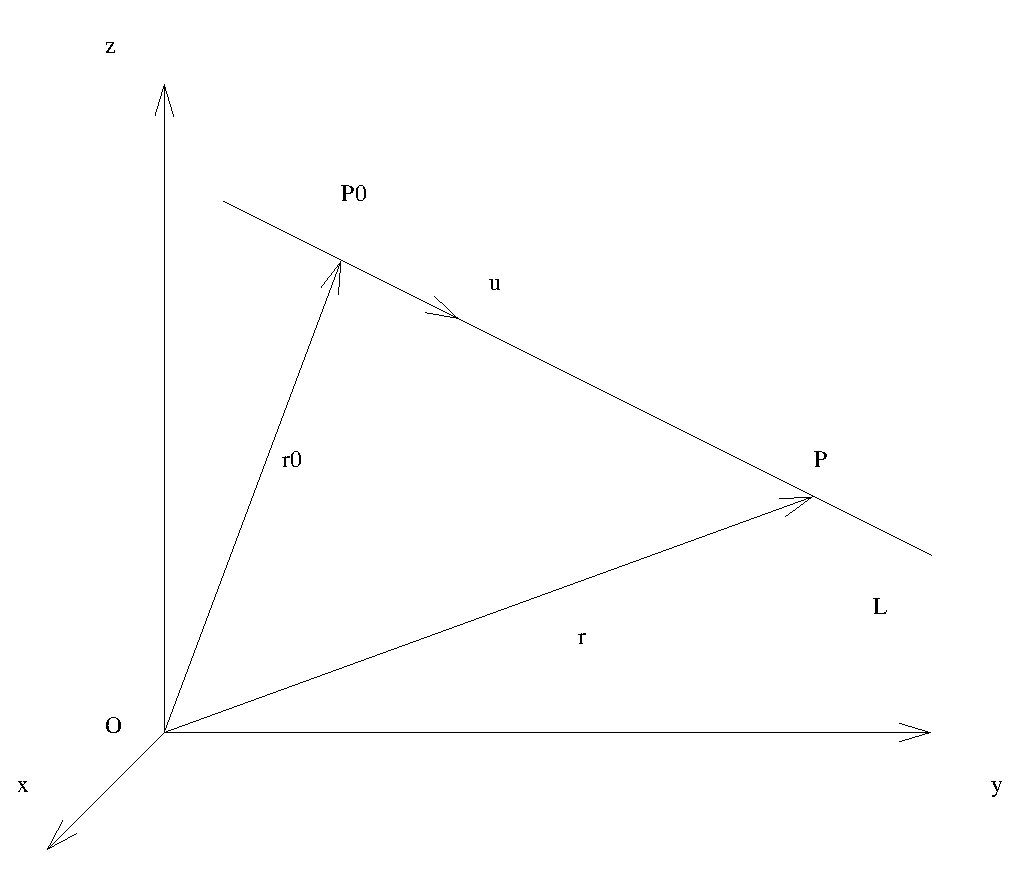
\includegraphics[height=2in]{../../modules/vectors/pictures/ok-line_point_direction_scalar.eps}
    \end{figure}
\end{columns}
\end{frame}

\begin{frame}
\uncover<1->{ $$\left\{ \begin{array}{ll}
           x & = x_0 + t u_1 \\
	   y & = y_0 + t u_2 \\
           z & = z_0 + t u_3
          \end{array}
\right. \Longrightarrow \boxed{\frac{x-x_0}{u_1} = \frac{y-y_0}{u_2} = \frac{z-z_0}{u_3}} \text{ \textcolor[rgb]{0.98,0.00,0.00}{Symmetric equations}}$$}

\uncover<2->{Caution! If $u_2=0$ (for example), then:
%
$$\frac{x-x_0}{u_1} = \frac{z-z_0}{u_3} \quad  \text{ and } \quad y=y_0 $$}

\uncover<3->{Example: Line with direction $\textbf{u} = \langle 4,5,6\rangle$ through $P_0(1,2,3)$:}
\begin{itemize}
 \item<4-> Parametric vectorial equation:
%
$$\textbf{r} = \langle 1,2,3\rangle + t \langle 4,5,6\rangle \leftrightarrow
\textbf{r} = \langle 1+4t, 2+5t, 3+6t\rangle$$
%
\item<5-> Parametric scalar equations:
%
$$\left\{ \begin{array}{ll}
           x & = 1 + 4t \\
	   y & = 2+5t \\
           z & = 3+6t
          \end{array}
\right. , \quad t \text{ real number.}$$
%
\item<6-> Symmetric equations:
%
$$\frac{x-1}{4} = \frac{y-2}{5} = \frac{z-3}{6}\; .$$
\end{itemize}

\end{frame}
\item \begin{frame}
 \frametitle{Line from Two Points}

\begin{columns}

\column{0.4\textwidth}
\psset{xunit=1.4cm, yunit=1.4cm}
\begin{pspicture}(-1,-0.4)(2,2.1)
\fcBoundingBox{-0.8}{-0.4}{4}{2.1}
\renewcommand{\fcScreen}{[-3 -1 -0.2] 0}
\tiny
\uncover<5->{\fcAxesIIId{2}{2}{2}}
\fcLineIIId{[0.5 0.5 1]}{[3 3 0.5]}
\fcLineIIId{[0.5 0.5 1]}{[4 4 0.3]}
\fcLineIIId[arrows=->]{[0 0 0]}{[1 1 0.9]}
\fcPutIIId[br]{[0.5 0.5 0.45]}{$\fcv r_0~$}

\fcLineIIId[linecolor=blue, arrows=->]{[1 1 0.9]}{[2.5 2.5 0.6]}
\fcPutIIId[br]{[1.75 1.75 0.8]}{$\fcv u$}

\fcLineIIId[arrows=->]{[0 0 0]}{[2.5 2.5 0.6]}
\fcPutIIId[b]{[1.25 1.25 0.3]}{$\fcv r_1$}

\fcDotIIId{[1 1 0.9]}
\fcPutIIId[lb]{[1 1 0.95]}{$P_0\uncover<5->{(x_0,y_0, z_0)} $}
\fcDotIIId{[2.5 2.5 0.6]}
\fcPutIIId[lb]{[2.5 2.5 0.65]}{$P_1\uncover<5->{(x_1, y_1, z_1)}$}
\fcDotIIId{[3.5 3.5 0.4]}
\fcLineIIId[arrows=->]{[0 0 0]}{[3.5 3.5 0.4]}
\fcPutIIId[b]{[1.75 1.75 0.2]}{$\fcv r$}
\fcPutIIId[b]{[3.5 3.5 0.5]}{$~P(x,y,z)$}
\fcPutIIId[t]{[4 4 0.3]}{$~L$}
\fcPutIIId[r]{[0 0 0.1]}{$O~~$}
\end{pspicture}
\column{0.6\textwidth}
\begin{itemize}
\item Given: distinct points $P_0$ and $P_1$, position vectors $\textbf{r}_0$ and $\textbf{r}_1$.
\item Goal: write equations of line $L$ through $P_0$ and $P_1$.
\item<2-> Direction of $L$: $\textbf{u} = \textbf{r}_1 - \textbf{r}_0$.
\item<5-> $\fcv{u} = \langle x_1-x_0,y_1-y_0,z_1-z_0\rangle$
\end{itemize}. 
\end{columns}
\uncover<3->{
\begin{definition}
\alert<1->{Parametric vectorial equation} of a line $L$:\\
$
\textbf{r} = \textbf{r}_0 + t(\textbf{r}_1-\textbf{r}_0)
\quad \Leftrightarrow \quad   \textbf{r} = (1-t)\textbf{r}_0 + t\textbf{r}_1
$

\uncover<5->{
\alert<1->{Parametric scalar equations} of a line $L$:
$\left|
\begin{array}{ll}
x & = x_0 + t(x_1-x_0) \\
y & = y_0 + t(y_1-y_0) \\
z & = z_0 + t(z_1-z_0)
\end{array}
\right. \Leftrightarrow \left| \begin{array}{ll}
x & = (1-t)x_0 + tx_1 \\
y & = (1-t)y_0 + ty_1 \\
z & = (1-t)z_0 + tz_1
\end{array}
\right. , \quad t \text{ real number.}$
} %uncover
\end{definition}
} %uncover
\end{frame}
\item \label{problemEquationsAllDiagonalsCubeContainingOrigin}
We recall that the 8 points $(1,1,1), (-1,1,1), (1,-1,1), (-1,-1,1), (1,1,-1)$, $(-1,1,-1), (1,-1,-1), (-1,-1,-1)$ (all possible sign combinations) give the vertices of a cube with edge 2 units.
 
Find equations for all lines connecting two vertices in the cube above that pass through the origin (how many connecting two vertices of a cube are there? How many of them are edges?).


\answer{ There are $4$ such edges. See the solution below for their equations.
}
\solution{\ref{problemEquationsAllDiagonalsCubeContainingOrigin}.
A cube has a total of $8 $ vertices. A line is given by two (distinct) points, therefore there are $\binom {8}{2}= \frac{8\cdot 7}{2}= 28$ total lines connecting two distinct vertices of a cube. Of those $12$ lines are cube edges, $12 = 6\cdot 2$ are diagonals of cube faces, and $4 $ are inner diagonals. All four inner diagonals contain the origin. A justification for this can undoubtedly be given by writing all $28$ line equations. However, the origin is in the center of the cube, and we know from our every-day geometric intuition that only the inner diagonals contain the center of a cube; we give no further justification.

The $4$ inner diagonals of the cube, call them $L_1, L_2, L_3, L_4$ pass through the points 

$\begin{array}{rcl}
(1,1,1), (-1,-1,-1) &\in& L_1\\
(1,1,-1), (-1,-1,1) &\in& L_2\\
(1,-1,1), (-1,1,-1) &\in& L_3\\
(-1,1,1), (1,-1,-1) &\in& L_4
\end{array}.
$

Therefore equations for these lines are given by:
$
\begin{array}{rl}
L_1:&  t\langle 1, 1, 1 \rangle\\
L_2:&  t\langle 1, 1, -1 \rangle\\
L_3:&  t\langle 1, -1, 1 \rangle\\
L_3:&  t\langle -1, 1, 1 \rangle\\
\end{array}
$.
}
\item Find an equation of the plane passing through the given point and with the given normal. Find parametric vectorial equations of the plane.

\begin{enumerate}
\item $P_0(2,3,5) $,  $\fcv n= \langle-3, -5, -7 \rangle$.
\item $P_0(1, 1, 1)$, $\fcv n= \langle 1,1,1 \rangle$.
\end{enumerate}
\solution{\ref{problemFindPlaneFromP(1,2,3)andn(4,5,6)}
As studied, an equation passing through $(1,2,3)$ and with normal $(4,5,6)$ has equation:

\[
\begin{array}{rcl}
\langle x, y, z\rangle\cdot \langle 4,5,6\rangle&=& \langle4,5,6\rangle\cdot \langle 1,2,3\rangle\\
4x +5y+6z&=&23
\end{array}
\]
To find parametric equations of the plane, we need to find two directions, $\fcv u, \fcv v$, that can be added to the base point to obtain all points in the plane. This means that a direction vector $\fcv u$ has to be perpendicular to $\fcv n$. Equivalently, a direction vector $\fcv u$ lies in the plane passing through the origin and orthogonal to $\fcv n$. This means $\fcv u\langle u_1, u_2, u_3\rangle$ satisfies the equation:
\begin{equation}\label{eqproblemFindPlaneFromP(1,2,3)andn(4,5,6)eq1}
\begin{array}{rcl}
\fcv u\cdot \fcv n&=&0\\
4 u_1+5u_2+6u_3&=&0.
\end{array}
\end{equation}
There are infinitely many solutions to that equation - in fact, for each point in the plane passing through the origin and orthogonal to $\fcv n$ there is one solution. However, we only need to find two such non-colinear solutions, and declare them to be our vectors $\fcv u$ and $\fcv v$. It is very easy to do that: if we set $u_1$ and $u_2$ to be arbitrary, then $u_3$ can always be chosen so as to make the equation above hold. There are a number of accepted ways to choose $u_1$ and $u_2$ in a not-so-arbitrary fashion. For reasons outside of the scope of this homework, such ways to choose $u_1$ and $u_2$ may be preferable to the choosing at random. Our scheme for choosing a vector $\fcv u$ will be to choose $u_1=1$ and $u_2=0$ (or the other way round for $\fcv v$), and then to rescale the resulting vector so all coordinates are integers and the first non-zero coordinate is positive. In other words, we select $\fcv u$ to be proportional to $\langle 1, 0, -\frac{4}{6} \rangle$, and $\fcv v$ to be proportional to $\langle 0, 1 ,-\frac{5}{6} \rangle$, i.e., we select
\[
\begin{array}{rcl}
\fcv u&=& \langle 3,0, -2 \rangle \\
\fcv v&=& \langle 0, 6, -5 \rangle
\end{array}. 
\] 
Finally we get that a parametric equation of the plane is given by:
\begin{equation}\label{eqproblemFindPlaneFromP(1,2,3)andn(4,5,6)eq2}
\langle 1,2,3 \rangle + s\langle 3,0, -2 \rangle +t\langle 0, 6, -5 \rangle\quad .
\end{equation}
The above equations are not unique; therefore our problem has many correct answers. 

A question arises: what do we need to do in order to check if two plane parametrizations are equivalent? Equivalently, how do we check that equation \eqref{eqproblemFindPlaneFromP(1,2,3)andn(4,5,6)eq2} gives a plane that coincides with the plane in given in \eqref{eqproblemFindPlaneFromP(1,2,3)andn(4,5,6)eq1}? Here's what we need to do to make sure our answer is correct (we leave the justification for that to the reader):
\begin{itemize}
\item Check that our $\fcv u, \fcv v$ are orthogonal to $\fcv n$. 
\item Check that our $\fcv u, \fcv v$ are not proportional to one another. 
\item Check that the base point of our equation is in the original plane. 
\end{itemize}

}
\item  Find an equation of plane $\mathcal P$ passing through the point and parallel to the given directions.

\begin{enumerate}
\item $P_0(1,2,3)$, $\fcv u=(2,3,5)$, $\fcv v=(3,5,7 )$.

\answer{$\mathcal P: z+y-4 x-1 =0$}
\item $P_0(1,1,1)$, $\fcv u=(1,-1,0)$, $\fcv v= (0,1,-1)$.
\answer{$\mathcal P:  z+y+x-3  =0$}
\end{enumerate}

\item \begin{frame}
 \frametitle{Plane from Three Points}

\begin{columns}
\column{0.4\textwidth}
\psset{xunit=0.8cm, yunit=0.8cm}
\begin{pspicture}(-0.2, -0.2)(3,3)
\tiny
\renewcommand{\fcScreen}{[-2 -1 -0.5] 0}
\fcParallelogramIIId{[-0.8 -0.8 3.6]}{[-1.4 2.4 1]}{[2.4 -1.4 1]}
\fcPutIIId[l]{[0 0 0.05]}{$~~O$}
\fcDotIIId{[0 0 0]}

\fcLineIIId[arrows=->, linestyle=dotted]{[0 0 0]}{[2 0 0]}
%\fcPutIIId{[1 0 0]}{$\fcv r_2$}
\fcLineIIId[arrows=->, linestyle=dotted]{[0 0 0]}{[0 2 0]}
%\fcPutIIId{[0 1 0]}{$\fcv r_0$}
\fcLineIIId[arrows=->, linestyle=dotted]{[0 0 0]}{[0 -0.4 2.4]}
%\fcPutIIId{[0 -0.2 1.2]}{$\fcv r_1$}
\fcDotIIId{[2 0 0]}
\fcDotIIId{[0 2 0]}
\fcDotIIId{[0 -0.4 2.4]}
\fcPutIIId[r]{[2 0 0]}{ $P_2(\fcv r_2)~$}
\fcPutIIId[tl]{[0 2 0]}{ $P_0(\fcv r_0)$}
\fcPutIIId[b]{[0 -0.4 2.4]}{ $P_1(\fcv r_1)$}
\fcLineIIId[arrows=->]{[0 2 0]}{[2 0 0]}
\fcPutIIId[t]{[1 1 -0.1]}{$~\fcv v$}
\fcLineIIId[arrows=->]{[0 2 0]}{[0 -0.4 2.4]}
\fcPutIIId[b]{[0 0.8 1.3]}{$~\fcv u$}%
\fcPerpendicularIIId{[4.8 6.8 4.8]}{ [0 2 0] [2 0 0]}{0.6}%
\fcPerpendicularIIId[arrows=<-]{[4.8 6.8 4.8]}{[0 2 0] [0 -0.4 2.4]}{0.6}%
\fcLineIIId[linestyle=dotted]{[0 0 0]}{[1.4 -0.84 1.44]}%
\fcPerpendicularIIId[arrows=<-]{[4.8 6.8 4.8]}{[0 2 0] [1.4 -0.84 1.44]}{0.8}%
\fcLineIIId[arrows=->]{[0 2 0]}{[1.4 -0.84 1.44]}%
\fcPutIIId[b]{[1.4 -0.84 1.44]}{$P(\fcv r)$}%
\end{pspicture}

\column{0.6\textwidth}
\begin{itemize}
\item Given: three non-collinear points $P_0(\fcv{r}_0)$, $P_1(\fcv{r}_1)$, $P_2(\fcv{r}_2)$.
\item Goal: find equations fo plane $\mathcal{P}$ passing through $P_0$, $P_1$, and $P_2$.
\item<2-> The plane is parallel to $\fcv{u} = \fcv{P}_0\fcv{P}_1 = \fcv{r}_1 -\fcv{r}_0$ and passing through $P_0$ $\Rightarrow$ this problem was solved previously.

\end{itemize}
\end{columns}
\only<3>{
Normal $\fcv{n} = \fcv{u} \times \fcv{v} =
(\fcv{r}_1-\fcv{r}_0) \times (\fcv{r}_2-\fcv{r}_0)$  \\

\alert<1->{Implicit equation}:
$$(\fcv{r}-\fcv{r}_0) \cdot \fcv{n} = 0$$
$$\boxed{(\fcv{r}-\fcv{r}_0) \cdot [(\fcv{r}_1-\fcv{r}_0) \times (\fcv{r}_2-\fcv{r}_0)] = 0}$$
$$\text{Vol}(R(\fcv{P}_0\fcv{P}, \fcv{P}_0\fcv{P}_1, \fcv{P}_0\fcv{P}_2)) = 0$$
}

\only<4>{
\alert<1->{Implicit equation}: $(\fcv{r}-\fcv{r}_0) \cdot [(\fcv{r}_1-\fcv{r}_0) \times (\fcv{r}_2-\fcv{r}_0)] = 0$

Let the points have coordinates $P_0(x_0,y_0,z_0)$, $P_1(x_1,y_1,z_1)$, $P_2(x_2,y_2,z_2)$. $P(x,y,z)$ is on plane $\mathcal{P}$:

\alert<1->{Implicit scalar equation}:
$\left| \begin{array}{ccc}
x-x_0 & y-y_0 & z-z_0 \\
x_1-x_0 & y_1-y_0 & z_1-z_0 \\
x_2-x_0 & y_2-y_0 & z_2-z_0
\end{array}
\right| = 0\; .$
}

\vskip 10cm
\end{frame}



\item Find the distance between the line and the point.

\begin{enumerate}
\item The line passing through $P_0(1,1,1)$ and $P_1(-1,-1,-1)$ and the point $Q(1,0,0)$.
\answer{$\frac{\sqrt{6}}{3} $}
\item The line passing through $P_0(-2,3,-5)$ and $P_1(3,4,5)$ and the point $Q(2,-2,2)$. 
\answer{$\frac{\sqrt{57610}}{42}$}
\end{enumerate}



\item Find the distance between the plane and the point.

\begin{enumerate}
\item The plane passing through $P_0(1,2,3) $, $P_1(2,3,5)$ and $P_2(3,5,7)$ and the point $Q(2,-2,2)$.
\answer{$\frac{3}{5}\sqrt{5}$}
\item The plane passing through $P_0(1,2,3) $, $P_1(2,3,5)$ and $P_2(3,5,7)$ and the point $Q(5,7,11)$.
\answer{$0$}
\item The plane passing through the points $P_0(1,1,1)$, $P_1(1,-1,-1)$, $P_2(-1,-1,1)$ and the point $Q(-1,1,-1)$.
\answer{$\frac{4}{3}\sqrt{3}$}
\end{enumerate}

\begin{comment}
Calculator code to solve above problem:

p0:=(1,2,3); 
p1:=(2,3,5);
p2:=(3,5,7);
q:=(2,-2,2);
u1:=p1-p0;
u2:=p2-p0;
u:=q-p0;
n:=u1\times u2;
((u n^t)_1)_1 /\sqrt{}(((n n^t)_1)_1) 
\end{comment}

\item Recall that a regular tetrahedron can be realized using 4 vertices of a cube. 

Find the angle between two edges of a regular tetrahedron. 
\item Recall that a regular tetrahedron can be realized using 4 vertices of a cube. 

Find the distance between two opposite edges of a regular tetrahedron inscribed in a 2x2x2 cm cube.
\item \begin{frame}
\frametitle{Distance between non-parallel lines}
\begin{columns}
\column{0.4\textwidth}
\begin{pspicture}(-2, -2)(2,2)
\tiny
\renewcommand{\fcScreen}{[-1 0 -0.5] 0}
\fcBoundingBox{-2}{-2}{2}{2}
\uncover<2->{%
\fcParallelogramIIId{[1.2 -1.2 1]}{[1.2 1.2 1]}{[-1.2 -1.2 1]}
\fcPutIIId[b]{[-1.2 -1.2 1]}{$\mathcal P$}
}%
\fcLineIIId{[-1 -1 -1]}{[1 1 -1]}
\fcLineIIId{[1 -1 1]}{[-1 1 1]} 
%\fcPerpendicularIIId[arrows=->, linecolor=green]{[0 0 -1]}{[1 -1 1] [-1 1 1]}{0.2}
\fcPutIIId[l]{[-1 1 1]}{$~~L_1$}
\fcPutIIId[r]{[-1 -1 -1.2]}{$L_2$}
\uncover<6->{%
\fcLineIIId[linestyle=dotted]{[0 0 1.3]}{[0 0 -1.3]}%
\fcPutIIId[rt]{[-0.1 0.1 -1]}{$Q_2~~~$}%
}%
\uncover<10->{%
\fcPerpendicularIIId[linestyle=none]{[0 0 -0.125]}{[0 0 1] [1 1 1]}{0.2}%
\fcPerpendicularIIId[linestyle=none]{[0 0 -0.125]}{[0 0 1] [-1 1 1]}{0.2}%
}%
\uncover<13->{%
\fcLineIIId[arrows=->, linecolor=green]{[0.8 -0.8 1]}{[0.9 0.9 -1]}%
\fcLineIIId[arrows=->, linecolor=green]{[0 0 1]}{[0.1 1.7 -1]}%
\fcDotIIId{[0.1 1.7 -1]}%
\fcPutIIId[l]{[0.1 1.7 -1]}{$~~R$}%
\fcPutIIId[l]{[0.05 0.85 0]}{$\fcv r_2- \fcv r_1$}%
}%
\uncover<6->{%
\fcPerpendicularIIId{[0.8 0.8 -1]}{[0 0 -1]}{0.2}
}%
\uncover<14->{\fcLineIIId[arrows=->, linecolor=brown]{[0.8 -0.8 1]}{[0 0 1]}%
\fcLineIIId[arrows=->, linecolor=brown]{[0.9 0.9 -1]}{[0.1 1.7 -1]}%
}%
\uncover<15->{%
\fcPerpendicularIIId{[0.1 1.7 -1]}{[0 0 -1]}{0.2}%
}%
\uncover<11->{%
\fcLineIIId[arrows=->, linecolor=blue]{[0 0 1]}{[0 0 -0.125]}%
\fcPutIIId[r]{[0 0 0.4375]}{$\fcv n~$}
}%
\uncover<4->{%
\fcLineIIId[linestyle=dotted]{[-1 -1 1]}{[1 1 1]}
\fcPutIIId[l]{[1 1 1]}{$~~L_2'$}
}%
\fcLineIIId[linecolor=red, arrows=->]{[0 0 -1]}{[0.75 0.75 -1]}
\fcPutIIId[t]{[0.325 0.325 -1.1]}{$\fcv u_2$}
\fcDotIIId{[0 0 -1]}
\uncover<12->{%
\fcDotIIId{[0.8 -0.8 1]}%
\fcPutIIId[br]{[0.8 -0.8 1]}{$P_1~$}%
\fcDotIIId{[0.9 0.9 -1]}%
\fcPutIIId[tr]{[0.9 0.9 -1]}{$P_2~$}%
}%
\uncover<5->{%
\fcDotIIId{[0 0 1]}
\fcPutIIId[r]{[-0.1 0.1 1]}{$Q_1~~~$}
}%
\fcLineIIId[linecolor=red, arrows=->]{[0 0 1]}{[-0.75 0.75 1]}
\fcPutIIId[br]{[-0.325 0.325 1]}{$\fcv u_1$}
\uncover<2->{
\fcLineIIId[linecolor=red, arrows=->]{[0 0 1]}{[0.75 0.75 1]}
\fcPutIIId[t]{[0.325 0.325 0.9]}{$\fcv u_2$}
}
%\fcPutIIId{[2 2 0]}{%
%\fcLineIIId[linecolor=red, arrows=->]{[0 0 1]}{[-0.75 0.75 1]}
%\fcPutIIId[br]{[-0.325 0.325 1]}{$\fcv u_1$}
%\fcLineIIId[linecolor=red, arrows=->]{[0 0 1]}{[0.75 0.75 1]}
%\fcPutIIId[t]{[0.325 0.325 0.9]}{$\fcv u_2$}
%}%
\end{pspicture}

\column{0.6\textwidth}
\begin{itemize}
\item Given: lines $\begin{array}{rrcl}L_1: & \fcv{r}&=& \fcv{r}_1+t\fcv{u}_1 \\ L_2:& \fcv{r} &=& \fcv{r}_2+s\fcv{u}_2\end{array}$
\item The lines are skew or intersecting, i.e., $\fcv{n} = \fcv{u}_1 \times \fcv{u}_2 \neq \fcv{0}$.
\item Goal: find distance between the lines = $d(L_1, L_2)$ = shortest distance b-n points on the two lines.
\end{itemize}
\end{columns}
\begin{itemize} 
\only<handout:1|1-8>{
\item<2-> Construct plane $\mathcal P$ with directions $\fcv u_1$, $\fcv u_2$ and passing through $L_1$. 
\item<3-> Distance b-n $L_2$ and points on $\mathcal P$ is constant.
\item<4-> Project $L_2$ orthogonally on $\mathcal P$; let the projection be $L_2'$.
\item<5-> Let $L_2' $ and $L_1$ intersect in point $Q_1$.
\item<6-> Let $Q_2$ be the heel of the perpendicular from $Q_1$ onto $Q_2$.
\item<7-> $\Rightarrow$ $Q_1Q_2=d(L_1, L_2)$.
}
\only<handout:1|8-16>{
\item \alert<8,9>{$|Q_1Q_2|=d(L_1, L_2)$}.
}
\only<handout:2|9-16>{
\item<10-> $\fcv Q_1\fcv Q_2 \perp L_1, L_2$ \uncover<11->{$\Rightarrow$  $\fcv Q_1 \fcv Q_2$ is proportional to $\fcv n = \fcv u_1\times \fcv u_2$.}
\item<12-> Pick arbitrary points on $L_1, L_2$ - say, the base points $P_1(\fcv r_1), P_2(\fcv r_2)$.
\item<13-> Let $R$ be such that $\fcv Q_1\fcv R=\fcv P_1 \fcv P_2=\fcv r_2-\fcv r_1$. 
\item<14-> Then $\fcv{P}_2\fcv R$ is proportional to $\fcv u_1$.
\item<15-> $\Rightarrow $ $\fcv Q_2\fcv R= \fcv Q_2  \fcv P_2+\fcv{P}_2\fcv{R}$ is perpendicular to $\fcv n$.
}
\only<handout:3|16->{
\item<16->\alert<16,17>{ $\Rightarrow$ $\fcv Q_1 \fcv Q_2= \fcv {proj} _{\fcv n} (\fcv r_2-\fcv r_1)$.}
}
\only<handout:3|17->{
\item<18-> 
$d(L_1,L_2)  = |\fcv{proj}_{\alert<19>{\fcv{n}}} (\fcv{r}_2-\fcv{r}_1)| \uncover<19->{= \boxed{\frac{|(\fcv{r}_2-\fcv{r}_1)\cdot \alert<19,20>{\fcv{n}} | }{ |\alert<19,20>{\fcv{n}}|}}} \uncover<20->{= \frac{ |(\fcv{r}_2 -\fcv{r}_1 )\cdot (\alert<20>{ \fcv{u}_1\times \fcv{u}_2})|}{ | \alert<20>{\fcv{u}_1\times \fcv{u}_2}|}}$
\item<21-> If lines are intersecting we know $d(L_1,L_2)=0$. \uncover<22->{Since the lines intersect $L_2$ and $L_2'$ coincide.} \uncover<23->{$\Rightarrow$ $(\fcv{r}_2-\fcv{r}_1) \cdot (\fcv{u}_1\times \fcv{u}_2) = 0$} \uncover<24->{$\Rightarrow $ the formula $d(L_1, L_2)= \frac{|(\fcv{r}_2 - \fcv{r}_1 )\cdot (\fcv{u}_1\times \fcv{u}_2)|}{ | \fcv{u}_1\times \fcv{u}_2|}=0$ produces the expected result.}
}
\end{itemize}

\vskip 5cm
\end{frame}


\solution{\ref{problemDistanceLineLine(1,2,3)(6,5,4)to(1,3,5)(2,4,6)}
We need to first establish whether the two lines are parallel. Let $\fcv u$ be the direction vector of the first line given by
\[\fcv u=\fcv Q_0 \fcv Q_1= ( 6,5,4)-( 1,2,3) = (5,3,1)
\]
and let $\fcv v$ be the direction vector of the second line given by
\[
\fcv v=\fcv P_0 \fcv P_1= (2,4,6 )-(1,3,5)=( 1, 1, 1).
\]
Now it is straightforward to see that the two lines are not parallel - indeed, one immediately sees that $\fcv u= (5,3,1)$ is not a scalar multiple of $\fcv v=(1,1,1)$. Since the two lines are not parallel, the two direction vectors determine a plane through the origin whose normal vector is given by
\[
\fcv n= \fcv u\times \fcv v=  (5,3,1)\times ( 1, 1, 1)= \left| \begin{array}{ccc} \fcv i & \fcv j &\fcv k\\ 5&3&1 \\1 &1 &1\end{array}\right|= 2\fcv i -4\fcv j+ 2\fcv k= (2, -4, 2)\quad .
\]
We note that if the vectors $\fcv u, \fcv v$ were parallel, then the cross product above would had been zero. Now the distance between the two lines is obtained by taking an arbitrary vector with tail on one line and head on the other, and computing the length of its projection it onto $\fcv n $. We use the vector $\fcv r= \fcv Q_0\fcv P_0$. Then the distance $d$ between the two lines is given by:
\[
d=\frac{|\fcv r \cdot \fcv n| }{|\fcv n|}= \frac{|\left(( 1,3,5) - ( 1,2,3)\right) \cdot \fcv  n|}{|\fcv n|}=\frac{ |( 0, 1, 2 )\cdot( 2, -4,2 )|}{|\fcv n|}=0.
\]
Therefore the distance between the two lines is zero. This completes our solution.

We note that since the distance between the lines is zero, they must intersect. As a consistency check for our work, let us verify that the two lines do indeed intersect. The first line is parametrized by $( 1,2,3)+t( 5,3,1) $ i.e., has parametric equations

\[
\left|\begin{array}{rcl}x&=& 1 +5t \\y&=&2+3t\\z&=&3+t \end{array}\right.\quad .
\]
Similarly, the second line is given by the equations
\[
\left|\begin{array}{rcl}x&=& 1 +s \\y&=&3+s\\z&=&5+s \end{array}\right.\quad .
\]
Therefore to find an intersection of the two lines, we need to solve the system
\[
\left|\begin{array}{rcl} 1 +5t&=&1+s \\2+3t&=&3+s\\3+t&=&5+s \end{array}\right.\quad.
\]
From the first equality we get that $s=5t$. We substitute that into the second equality to get that $t=-\frac{1}{2}$. Therefore the intersection of the two lines is the point

\[
(1,2,3)-\frac{1}{2}(5,3,1)= \left(-\frac{3}{2}, \frac{1}{2}, \frac{5}2\right)= (1,3,5)-\frac{5}{2}(1,1,1)\quad ;
\]
all our error checks have been successful.
}

\solution{\ref{problemDistanceLineLine(1,3,4)(2,3,1)to(1,2,2)(0,2,5)}
We present a solution in a concise form suitable for exam taking.

Let $L_1, L_2$ be the two lines.
\[
\begin{array}{rcll|l}
\fcv u &=& (2,3,1)-(1,3,4)=(1,0,-3)&& \text{direction vector } L_1\\
\fcv v &=& (0,2,5)-(1,2,2)=(-1,0,3)=-\fcv u&&\text{direction vector } L_2\\
&&\text{Therefore } L_1 \parallel  L_2\\
\fcv r&=&(2,3,1)-(0,2,5)=(2,1,-4) &&\text{arbitrary vector connecting } L_1, L_2\\
L_1\parallel L_2\Rightarrow\\
\text{dist}(L_1,L_2)&=&|\fcv{orth}_{\fcv u} \fcv r| \\
&=&\left|\fcv r- \fcv {proj}_{\fcv u} \fcv r \right|\\
&=&\left|\fcv r- \frac{\fcv r \cdot \fcv u}{|\fcv u|^2}\fcv{u} \right|\\
&=&\left| (2,1,-4)-\frac{(2,1,-4)\cdot (1,0,-3)}{1^2+0^2+(-3)^2}(1,0,-3) \right|\\
&=&\left|\left(\frac{3}{5}, 1, \frac{1}{5} \right)\right|\\
&=&\sqrt{\left(\frac{3}{5}\right)^2+ 1^2+ \left(\frac{1}{5}\right)^2 }\\
&=&\frac{\sqrt{35}}{5} \quad .
\end{array}
\]
}

\solution{\ref{problemDistanceLineLine(1,3,4)(2,3,1)to(1,2,2)(0,2,4)}
We present a solution in a concise form suitable for exam taking.
\[\begin{array}{rcll|l}
\fcv u &=& (2,3,1)-(1,3,4)=(1,0,-3)&& \text{direction vector } L_1\\
\fcv v &=& (0,2,4)-(1,2,2)=(-1,0,2)=-\fcv u&&\text{direction vector } L_2\\
\fcv r &=& (1,3,4)-(1,2,2)=(0, 1, 2)  &&\text{arbitrary vector connecting } L_1,L_2\\
\fcv n&=&u\times v=(0, 1, 0) &&\neq 0\Rightarrow L_1\not \parallel L_2\\
L_1\not \parallel L_2\Rightarrow \\
\text{dist}(L_1,L_2)&=&\left|\fcv {proj}_{\fcv n} \fcv r\right|\\
&=&\left|\fcv r \cdot \frac{\fcv n}{|\fcv n|}\right|\\
&=&\left| (0,1,2)\cdot (0,1,0)\right|\\
&=&1\quad .
\end{array}
\]
}

\item Find the angle between the line and the plane.

\begin{itemize}
\item The line passing through $(-1,-1,-1) $ and $(1 , 1, 1)$ and the plane with equation $z=-1$.
\item The line passing through $(2,3, 5)$ and $(3,5,7)$ and the plane passing through $(1,0,0)$, $(0,1,0)$ and $(0,0,1)$.
\end{itemize}
\item Recall that a regular tetrahedron can be realized using 4 vertices of a cube. Find the angle between an edge of a regular tetrahedron and one of the two sides of the tetrahedron not containing the edge.
\item Recall that a regular tetrahedron can be realized using 4 vertices of a cube.

Find the angle between two faces of a regular tetrahedron.
\homeworkEnd
\end{comment}

%\begin{comment}
\homeworkStart{on Lecture 5 \\Will be quizzed: date to be announced\\ the partial answer key has not been proofread, use with caution}{}
\item Find polar equations of the line given below.

\begin{enumerate}[ref={\fcProblemRef}]
\item The line $x+y=1$.
\answer{$\begin{array}{rcl} r(\cos \theta +\sin \theta)&=&1 \\ r=\frac{\sqrt{2}}{2}\sec \left(\theta -\frac{\pi}{4}\right) \end{array} $}
\item \label{problemWriteInPolarx+sqrt(3)y=2} The line $ x+\sqrt{3}y=2$.
\answer{ $\begin{array}{rcl} r\left(\frac{1}{2}\cos \theta +\frac{\sqrt{3}}{2}\sin \theta\right)&=& 1 \\ r=\sec \left(\theta-\frac{\pi}{3} \right) \end{array}$}
\item The line passing through $(3,5)$ and $(5,7)$.

\answer{$\begin{array}{rcl} x-y&=&-2\\ r(\cos \theta -\sin \theta)&=&-2\\ r=-\sqrt{2}\sec\left(\theta+\frac{\pi}{4} \right) \end{array} $}
\item The line passing through $(2,3)$ and $(-3,-2)$.
\answer{$\begin{array}{rcl} x-y&=&-1\\ r(\cos \theta -\sin \theta)&=&-1\\ r=-\frac{\sqrt{2}}{2} \sec \left( \theta + \frac{ \pi }{4} \right) \end{array} $}
\end{enumerate}
\item \solution{\ref{problemWriteInPolarx+sqrt(3)y=2}

Polar coordinates are given by
\[
\left|\begin{array}{rcl}
x&=& r\cos \theta\\
y&=& r\sin \theta 
\end{array}\right. .
\]
All we need to do to obtain polar equations for our line is substitute the above expressions in the equation for the line. 
\[
r\cos \theta + \sqrt{3}r\sin \theta= 2.
\]
This is a perfectly good answer, but we can transform the equation to make it look more compact:
\[
\begin{array}{rcll|l}
\displaystyle r\cos \theta + \sqrt{3}r\sin \theta&=&\displaystyle 2\\
\displaystyle r\underbrace{\frac{1}{2}}_{=\cos \left(\frac{\pi}{3}\right)} \cos\theta +r \underbrace{\frac{\sqrt{3}}{2}}_{=\sin \left(\frac{\pi}{3}\right)} \sin\theta &=&\displaystyle  1 \\
\displaystyle r\cos \left(- \frac{\pi }{3}\right)\cos \theta -\sin \left(- \frac{\pi }{3}\right)\sin \theta &=& 1&&   \text{use } \cos (a+b)= \cos a \cos b - \sin a \sin b\\
\displaystyle r\cos (\theta -\frac{\pi}{3})&=&1\\
r&=&\displaystyle \frac{1}{\cos \left(\theta - \frac{\pi}{3} \right)}\\
&=&\displaystyle \sec\left (\theta - \frac{\pi}{3}\right )\quad .

\end{array}
\]


}
\item Find polar equations of the circle given below.

\begin{enumerate}
\item The circle given by $(x-1)^2+y^2=1$.
\answer{$r=2\cos \theta$}
\item The circle given by $x^2+ x+y^2=1$.
\answer{$r^2+r\cos \alpha -1=0$}
\item The circle with center $(1,2)$ and radius $3$.
\answer{$r^{2} -4 r \sin{}\theta-2 r \cos{}\theta-4 =0$}
\item The circle with center $(2,3)$ and radius $4$.
\answer{$r^{2} -6 r \sin{}\theta-4 r \cos{}\theta-3 =0$}
\end{enumerate}
\item Find an equation of the plane in cylindrical coordinates.

\begin{enumerate}
\item The plane given by $x+y+z=1$.
\item The plane given by $2x+3y-5z=0$.
\item The plane passing through $(-1, 1, 1)$, $(1, 1, -1)$ and $(1, -1, 1)$.
\item The plane passing through $(2,3,5 )$, $(3, 5, 2)$ and $(5, 2, 3)$.
\end{enumerate}
\item Find an equation of the sphere in cylindrical coordinates.

\begin{enumerate}
\item The unit sphere.
\item The sphere with equation $x^2 +x+ y^2+2y + z^2 +3z=0$.
\item The sphere with center $(1,2,3)$ and radius $5$.
\end{enumerate}
\item Find an equation of the plane in spherical coordinates.

\begin{enumerate}
\item The plane given by $x+y+z=1$.
\item The plane given by $2x+3y-5z=0$.
\item The plane passing through $(-1, 1, 1)$, $(1, 1, -1)$ and $(1, -1, 1)$.
\item The plane passing through $(2,3,5 )$, $(3, 5, 2)$ and $(5, 2, 3)$.
\end{enumerate}
\item Find an equation of the sphere in spherical coordinates.

\begin{enumerate}
\item The unit sphere.
\item The sphere with equation $x^2 +x+ y^2+2y + z^2 +3z=0$.
\item The sphere with center $(1,2,3)$ and radius $5$.
\end{enumerate}

\homeworkEnd
\end{comment}

%\begin{comment}
\homeworkStart{on Lecture 7}{quiz time to be announced in class}
%\item Match the surface graph to its mathematical name and to its equation.

\begin{enumerate}
\item
\begin{pspicture}(-2,-2)
\renewcommand{\fcScreen}{[-2 -1 -0.9] 0}
\fcSurfaceDirectDraw{}{-1}{-1}{1}{1}{[u v u u mul v v mul add]}
\end{pspicture}

\end{enumerate}
\item Determine the type of the quadratic surface given by the equation.
\begin{enumerate}
\item 
$x^2 +y^2+z^2+x+2y+3z=0$.
\answer{sphere (also ellipsoid)}
\item $x^2 +2y^2+z^2+x+2y+3z=0$.
\answer{(circular) ellipsoid}
\item $x^2 +2y^2+3z^2+x+2y+3z=0$.
\answer{ellipsoid}
\item \label{problemTypeOfSurfacez^2+2y^2-3x^2+x+y+1=0} $z^2+2y^2-3x^2 + x+y+1=0 $.
\answer{(elliptic) hyperboloid one sheet}
\item $z^2-y^2+\frac{1}{4}x^2 + x-y+1=0 $.
\answer{(elliptic) hyperboloid two sheets}
\item $x^2+y^2-\frac{1}{4}z^2 + x-y+5=0 $.
\answer{(circular) hyperboloid one sheet}
\item $\frac{1}{4}x^2-y^2+z^2-x+1=0$
\answer{(elliptic) cone}
\item $-\frac{1}{4}x^2+y^2+z^2-x-1=0$
\answer{(circular) cone}
\item $xy +z^2+1=0$. Hint: write $x=\frac{1}{\sqrt{2}}(u+v)$, $y=\frac{1}{ \sqrt{ 2} } (u-v) $ for some new variables $u,v$. Solve the problem in the $z,u,v$ -coordinates. Argue that the (axes of the) $u,v,z$-coordinate system can be obtained from the $x,y,z$-coordinate system via rotation.
\answer{(circular) hyperboloid one sheet}
\item $x^2+2y^2+z=0 $.
\answer{(elliptic) paraboloid}
\item $x^2+y^2+2xy+z=0 $.
\answer{cylindrical paraboloid}
\item $x^2-y^2+2x+z=0 $.
\answer{parabolic hyperboloid}
\end{enumerate}
\homeworkEnd

%\end{comment}


\begin{comment}
\homeworkStart{on Lecture 6 \\Will be quizzed: time to be announced in class}{}
\item 
Integrate 
\[
\int \frac{x }{2x^2+x-1}\diff{}x
\]

\solution{
The quadratic in the denominator has real roots and therefore factors using real numbers. Therefore we have to use the partial fractions algorithm.
\[
\begin{array}{rcll|l}
\displaystyle \int \frac{x }{2x^2+x-1}\diff{}x&=&\displaystyle \frac{1}{2}\int \frac{x}{\left( x+1\right)\left(x-\frac{1}{2}\right)} \diff x &&\text{partial fractions, see below}\\
&=&\displaystyle  \frac{1}{2}\int \frac{x}{\left( x+1\right)\left(x-\frac{1}{2}\right)} 
\end{array}
\]
}
\item 
Evaluate the indefinite integral. Illustrate all steps of your solution. 
\begin{enumerate}
\item (3 points) $\int \frac1{x^2+x+1}dx$
\item (3 points) $\int \frac1{4x^2+4x+1}dx$
\item (3 points) $\int \frac1{2x^2+5x+1}dx$
\item (5 points) $\int \frac{15x^2-4x-81}{(x-3)(x+4)(x-1)}dx$
\item (5 points) $\int \frac {x^{4}+10x^{3}+18x^{2}+2x-13}{x^{4}+4x^{3}+3x^{2}-4x-4}dx$ 

Check first that $(x-1)(x+2)^2(x+1)= x^{4}+4x^{3}+3x^{2}-4x-4$. \end{enumerate}
\homeworkEnd
\end{comment}

\begin{comment}
\homeworkStart{on Lecture 7 \\Will be quizzed: time to be announced in class}{}
\item 
Integrate.
\begin{multicols}{2}
\begin{enumerate}[ref={\fcProblemRef}]
\item \label{problemInt1/(3+cos x)dx} $\displaystyle \int \frac{1}{3+\cos x}\diff x$.

\answer{$\displaystyle\frac{1}{\sqrt{2}} \Arctan \left( \frac{ 1}{ \sqrt{2}} \tan \left( \frac{x }{2} \right)\right)+C$}
\item $\displaystyle \int \frac{1}{4+\cos x}\diff x$.

\answer{$\displaystyle  \frac{2}{15}\sqrt{15} \Arctan{}\left(\frac{\sqrt{15}}{5}\tan\left(\frac{x}{2}\right)\right)+C$}
\item $\displaystyle \int \frac{1}{3+\sin x}\diff x$.

\answer{$\displaystyle \frac{1}{\sqrt{2}} \Arctan \left(\frac{3 \tan \left(\frac{x}{2} \right)+1 }{2\sqrt{2}}\right) +C$}
\item \label{problemInt1/(2+tan x)dx}$\displaystyle \int \frac{1}{2+\tan x}\diff x$.  (Hint: this integral can be done simply with the substitution $x=\Arctan t$.)

\answer{$\displaystyle \frac{1}{5} \ln \left(\sin x+2\cos x\right)+\frac{2}{5}x+C$}

\item \label{problemint1/(2sinx-cosx+5)dx} $\displaystyle \int \frac{ \diff x }{ 2\sin x - \cos x +5}$.


\answer{$\displaystyle \frac{ \sqrt{5}}{5}\Arctan \left( \frac{3}{ \sqrt{5}} \left({ \tan \left(\frac{\theta}{2} \right)}+\frac{1}{3} \right) \right)+C$}
\end{enumerate}
\end{multicols}
Integrate.
\begin{enumerate}
\item $\displaystyle \int \sin (3 x) \cos (2x)\diff x$.
\item $\displaystyle \int \sin x \cos (5x)\diff x$.
\item $\displaystyle \int \cos (3x) \sin (2x)\diff x$.
\end{enumerate}

Integrate.
\begin{multicols}{2}
\begin{enumerate}[ref={\fcProblemRef}]
\item $\displaystyle \int \sin^2 x \cos x\diff x$.

\answer{$ \frac{1}{3}\sin^3 x+C$}

\item $\displaystyle \int \sin^2 x\diff x$.

\answer{$ \frac{x}{2} -\frac{1}{4}\sin (2x) +C$}
\item $\displaystyle \int \cos^3 x\diff x$.

\answer{$ \sin x -\frac{1}{3}\sin^3 x+C$}


\item 
$\displaystyle \int \sin^3 x \cos^4 x\diff x$.

\answer{$ \frac{1}{7} \cos^{7}{}x-\frac{1}{5} \cos^{5}{}x +C$}

\end{enumerate}
\end{multicols}
Integrate 
\begin{enumerate}
\item $\displaystyle \int \sec^3x  \diff x$.
\item $\displaystyle \int \tan^3x \diff x$.
\item $\displaystyle \int \sec^2x\tan^2x \diff x$.

\end{enumerate}

\homeworkEnd
\end{comment}

\begin{comment}
\homeworkStart{on Lecture 8 \\Will be quizzed: date to be announced}{}
\item Compute the integral.

\begin{enumerate}[ref={\fcProblemRef}]
\item \label{problemIntegratesqrt(x^2+1)dx}
$\displaystyle
\int \sqrt{x^2+1}\diff x
$

\answer{$\frac{1}{2}x\sqrt{x^2+1}+\frac{1}{2}\ln\left( \sqrt{x^2+1}+x\right)+C $}

\item $\displaystyle
\int \sqrt{x^2+2}\diff x
$

\answer{$ \ln{}\left(\sqrt{\frac{1}{2} x^{2}+1}+\frac{\sqrt{2}}{2} x\right)+\frac{\sqrt{2}}{2} x \sqrt{\frac{1}{2} x^{2}+1}+C$}

\item 
$\displaystyle
\int \sqrt{x^2+x+1}\diff x
$

\answer{$\frac{3}{4} \left(\frac{1}{2} \ln{}\left(\sqrt{\frac{4}{3} (x+\frac{1}{2})^{2}+1}+\frac{2}{3}\sqrt{3} \left(x+\frac{1}{2}\right)\right)+\frac{\sqrt{3}}{3} \left(x+\frac{1}{2}\right) \sqrt{\frac{4}{3} (x+\frac{1}{2})^{2}+1}\right)  +C$}
\item \label{problemIntegrate sqrt(2x^2+2x+1)dx}
$\displaystyle
\int \sqrt{\left(2x^2+2x+1\right)}\diff x
$

\answer{$\frac{\sqrt{2}}{4} \left( \frac{1}{2} (2x+1)\sqrt{(2x+1)^2+1 }+ \frac{1}{2}\ln \left( \sqrt{(2x+1)^2+1 }+2x+1\right) \right)+C$}

\item \label{problemIntegrate sqrt(3x^2+2x+1)dx}
$\displaystyle
\int \sqrt{\left(3x^2+2x+1\right)}\diff x
$

\answer{$
\begin{array}{l}
\frac{2}{9}\sqrt{3} \left(\frac{1}{2} \ln{}\left(\sqrt{\frac{9}{2} (x+\frac{1}{3})^{2}+1}+\frac{3}{2}\sqrt{2} \left(x+ \frac{1}{3} \right)\right)\right. \\\left. +\frac{3}{4}\sqrt{2} \left(x+\frac{1}{3}\right) \sqrt{\frac{9}{2} (x+\frac{1}{3})^{2}+1}\right) +C \end{array}$}

\item \label{problemintsqrt(x^2+1)/(x+1)dx}
$\displaystyle\int \frac{\sqrt{x^2+1}}{x+1}\diff x $

\answer{$ \begin{array}{l} -\sqrt{2} \ln{}\left(\sqrt{x^{2}+1}- x+\sqrt{2}-1\right) \\
+\sqrt{2} \ln{}\left(\sqrt{x^{2}+1}- x-\sqrt{2}-1\right)\\
+ \ln{} \left( \sqrt{x^{2}+1}- x\right)\\
+ \sqrt{x^{2}+1}
\end{array}
$}
\end{enumerate}

\item Integrate
\begin{enumerate}[ref={\fcProblemRef}]
\item  \label{problemintsqrt(1-x^2)dx}
$\displaystyle
\int \sqrt{1-x^2}\diff x$

\answer{$ $}
\item 
$\displaystyle
\int \sqrt{2-x^2}\diff x
$
\item 
$\displaystyle
\int \sqrt{-x^2+x+1}\diff x
$
\item 
$\displaystyle
\int \sqrt{2-x-x^2}\diff x
$

\item \label{problemintsqrt(1-x^2)/(1+x)dx}
$\displaystyle
\int \frac{\sqrt{1-x^2} }{1+x}\diff x
$
\item 
$\displaystyle
\int \frac{\sqrt{1-x^2} }{2+x}\diff x
$
\end{enumerate}
\item Integrate
\begin{enumerate}[ref={\fcProblemRef}]
\item 
\[
\int \sqrt{x^2-1}\diff x
\]
\item 
\[
\int \sqrt{x^2-2}\diff x
\]
\item 
\[
\int \sqrt{2x^2+x-1}\diff x
\]
\item 
\[
\int \sqrt{x^2+x-1}\diff x
\]
\end{enumerate}

\homeworkEnd
\end{comment}

\begin{comment}
\homeworkStart{on Lecture 9 \\Quiz time to be announced in class}{}
\item Compute the limits. The answer key has not been fully proofread, use with caution.
\begin{multicols}{2}
\begin{enumerate}
\item $\displaystyle \lim\limits_{x\to 0} \frac{\sin x  }{x}$. 

\answer{$1$}
\item $\displaystyle \lim\limits_{x\to 0} \frac{x}{\ln (1+x)}$. 

\answer{$ 1$}
\item $\displaystyle \lim\limits_{x\to 0} \frac{x^2}{x-\ln (1+x)}$. 

\answer{$2$}
\item $\displaystyle \lim\limits_{x\to 0} \frac{x^2}{\sin x\ln (1+x)}$. 

\answer{$ 1$}
\item $\displaystyle \lim\limits_{x\to 0} \frac{\sin^2 x  }{\left(\ln (1+x)\right)^2}$.

\answer{$ 1$}
\item $\displaystyle \lim\limits_{x\to 0} \frac{\cos x- 1}{\sin x\ln (1+x)}$.

\answer{$- \frac{1}{2} $}
\item $\displaystyle \lim\limits_{x\to 0} \frac{\arctan x -x}{x^3} $.

\answer{$ -\frac{1}{3} $}
\item $\displaystyle \lim\limits_{x\to 0} \frac{\arcsin x -x}{x^3} $.

\answer{$ \frac{1}{6}$}
\item $\displaystyle \lim\limits_{x\to 1} \frac{x}{x-1}-\frac{1}{\ln x}$.

\answer{$ \frac{1}{2}$}
\item $\displaystyle \lim\limits_{x\to 0} \frac{\cos (nx) -\cos (mx)}{x^2 }$.

\answer{$\frac{m^2-n^2}2 $}
\item \label{eqProblemLimlixto0(arcsinx-x-x^3/6)/(sin^5 x)}  $\displaystyle \lim \limits_{x\to 0} \frac{\arcsin x-x-\frac{1}{6}x^3}{\sin^5 x} $. 

\answer{$\frac{3}{40}$}
\item \label{problemLHospital (sin (pi x) ln x )/ (cos pi x +1)}  $\displaystyle \lim\limits_{x\to 1} \frac{\sin \left(\pi x \right)\ln x }{\cos(\pi x)+1 } $.

\answer{$-\frac{2}{\pi}$}

\item $\displaystyle \lim\limits_{x\to 0} \frac{\sin x-x }{\arcsin x-x } $.

\answer{$ -1$}
\item \label{problemlim x to 0 (sin x - x)/(arctan x - x)} $\displaystyle \lim\limits_{x\to 0}\frac{\sin x- x}{\Arctan x -x}$.

\answer{$\frac{1}{2}$}

\item 
\label{problemlimxtoinftysin(2/x)}
$ {\displaystyle \lim_{x \to \infty} x \sin\left(\frac{2}{x}\right)}.$

\answer{$2$}

\end{enumerate}
\end{multicols}
The very last problem can be done easily using Maclaurin series, but we challenge the student to try it using L'Hospital's rule. This problem is solved in Chapter 9 of the Calculus notes ``Calculus for beginners''.
\homeworkEnd
\end{comment}
\begin{comment}
\homeworkStart{on Lecture  10\\ will be quizzed: date to be announced in class}{}
\item Determine whether the integral is convergent or divergent. Motivate your answer.
\begin{multicols}{2}
\begin{enumerate}[ref={\fcProblemRef}]
\item $\displaystyle \int\limits_{2}^{\infty}\frac{1}{(x-1)^{\frac32}} \diff x$.

\answer{convergent}
\item $\displaystyle \int\limits_{-1}^{1}\frac{1}{\sqrt[5]{1+x}} \diff x$.

\answer{convergent}
\item $\displaystyle \int\limits_{1}^{\infty }\frac{1}{\sqrt[5]{1+x}} \diff x$.

\answer{divergent}
\item $\displaystyle \int\limits_{-1}^{\infty }\frac{1}{\sqrt[5]{1+x}} \diff x$.

\answer{divergent}
\item $\displaystyle \int\limits_{-\infty }^{0}\frac{1}{2-3x} \diff x$.

\answer{divergent}
\item $\displaystyle \int\limits_{-\infty }^{0}\frac{1}{(2-3x)^{2}} \diff x$.

\answer{convergent}
\item $\displaystyle \int\limits_{-\infty }^{0}\frac{1}{(2-3x)^{1.00000001}} \diff x$.

\answer{convergent}
\item $\displaystyle \int\limits_{-2}^{ \frac{1}{ 2}} \frac{1}{2x-1} \diff x$.

\answer{divergent}

\item $\displaystyle \int\limits_{-1}^{\infty} e^{-3x} \diff x$.

\answer{convergent, equals $\frac{e^{3}}{3}$}

\item $\displaystyle \int\limits_{-\infty }^{5}  2^x \diff x$.

\answer{convergent}
\item $\displaystyle \int\limits_{-\infty }^{\infty}x^3 \diff x$.

\answer{divergent}
\item $\displaystyle \int\limits_{-\infty}^{\infty} x e^{-x^2} \diff x$.

\answer{convergent, equals $0$}

\item \label{problemConvergencesqrt(x)e^-sqrt(x)zerotoinfty} $\displaystyle \int\limits_{0}^{\infty} \sqrt{x} e^{-\sqrt{x}} \diff x$.

\answer{convergent, equals $4 $}

\item $\displaystyle \int\limits_{0}^{\infty}\sin^2 x \diff x$.

\answer{divergent}
\item $\displaystyle \int\limits_{0}^{5}\frac{1}{x^2+x-2} \diff x$.

\answer{divergent}
\item $\displaystyle \int\limits_{0}^{\infty}\frac{1}{x^2+x+1} \diff x$.

\answer{convergent}
\item $\displaystyle \int\limits_{2}^{\infty}\frac{1}{x^2-x-1} \diff x$.

\answer{convergent}
\item $\displaystyle \int\limits_{0}^{\infty}\frac{1}{x^2-x-1} \diff x$.

\answer{divergent}
\item \label{problemConvergencex^2/(x^4+2)from-inftyto+infty}

$\displaystyle \int\limits_{-\infty}^{\infty} \frac{x^2}{x^4+2} \diff x$.
\answer{convergent}

\item 
$\displaystyle \int\limits_{100}^{\infty} \frac{1}{x\ln x} \diff x$.

\answer{divergent}

\item $\displaystyle \int\limits_{100}^{\infty} \frac{1}{x(\ln x)^2} \diff x$.

\answer{convergent}
\item $\displaystyle \int\limits_{0}^{1}\ln x \diff x$.

\answer{convergent}
\item $\displaystyle \int\limits_{0}^{1}\frac{\ln x}{\sqrt{x}} \diff x$.

\answer{convergent}
\item $\displaystyle \int\limits_{0}^{2}x^3\ln x \diff x$.

\answer{convergent, equals $-1+4 \ln 2 $}

\item $\displaystyle \int\limits_{0}^{1} \frac{e^{\frac{1}{x}}}{x^2} \diff x$.

\answer{divergent}
\item $\displaystyle \int\limits_{-1}^{0} \frac{e^{\frac{1}{x}}}{x^2} \diff x$.

\answer{convergent}

\end{enumerate}
\end{multicols}

\item Determine whether the integral is convergent or divergent. Motivate your answer. The answer key has not been proofread, use with caution.

\begin{multicols}{2}
\begin{enumerate}
\item $\displaystyle \int\limits_{100}^{\infty} \frac{1}{x\ln x} \diff x$.
\answer{divergent}
\item $\displaystyle \int\limits_{100}^{\infty} \frac{1}{x(\ln x)^2} \diff x$.
\answer{convergent}
\item $\displaystyle \int\limits_{0}^{1}\ln x \diff x$.
\answer{convergent}
\item $\displaystyle \int\limits_{0}^{1}\frac{\ln x}{\sqrt{x}} \diff x$.
\answer{convergent}
\item $\displaystyle \int\limits_{0}^{2}x^3\ln x \diff x$.
\answer{convergent}
\item $\displaystyle \int\limits_{0}^{1} \frac{e^{\frac{1}{x}}}{x^2} \diff x$.
\answer{divergent}
\item $\displaystyle \int\limits_{-1}^{0} \frac{e^{\frac{1}{x}}}{x^2} \diff x$.
\answer{convergent}
\item $\displaystyle \int \limits_{0}^{\infty}\sin x^2\diff x$ (This problem is more difficult and may require knowledge of sequences to solve).
\answer{convergent}
\end{enumerate}
\end{multicols}

\homeworkEnd
\end{comment}

\begin{comment}
\homeworkStart{on Lecture 11 \\Will be quizzed on Wednesday}{}
\item List the first 4 elements of the sequence. 
\begin{multicols}{2}
\begin{enumerate}
\item $\displaystyle a_n= \frac{(-1)^n}{n}$.
\item $\displaystyle a_n=\frac{1}{n!}$.
\item $\displaystyle a_n=\cos (\pi n)$.
\item $\displaystyle a_n=\frac{(-1)^n}{2n+1}$.
\item $\displaystyle a_n=\frac{\sqrt{5}}{5}\left( \left(\frac{1+\sqrt{5 }}{2} \right)^n- \left(\frac{1-\sqrt{5}}{2}\right)^n\right) $
\end{enumerate}
\end{multicols}
\item List the first 5 elements of the sequence. 
\begin{multicols}{2}
\begin{enumerate}
\item $\displaystyle a_{n+1}=\frac{1}{2}\left(a_n+ \frac{3}{a_n}\right)$.
\item $\displaystyle a_n=a_{n-1}+a_{n-2}$, $a_1=1$, $a_2=1$.
\item $\displaystyle a_n= \frac{\left(\frac{1}{2}-n\right)}{n} a_{n-1} $, $a_0=1$.
\item $\displaystyle a_n= a_{n-1}+2n+1$, $a_0=1$.
\item $\displaystyle a_n:=\frac{1}{n} a_n$.
\end{enumerate}
\end{multicols}
\item Give a simple sequence formula that matches the pattern below. 

\begin{multicols}{2}
\begin{enumerate}
\item $\displaystyle \left(1, \frac{1}{3}, \frac{1}{5}, \frac{1}{7},\frac{1}{9},\dots \right)$.

\answer{$a_n=\frac{1}{2n-1}$}
\item $\displaystyle \left(-1, \frac{1}{5}, -\frac{1}{25}, \frac{1}{125},-\frac{1}{625}, \frac{1}{3125}\dots \right)$

\answer{$a_n=\left(-\frac{1}{5}\right)^{n-1}$}
\item $\displaystyle \left(-5, 2, -\frac{4}{5}, \frac{8}{25}, -\frac{16}{125}, \frac{32}{625},\dots \right)$

\answer{$a_n=-5\left(-\frac{2}{5}\right)^{n-1}$}

\item $\displaystyle \left(4, 7, 10, 13, 16, 19,\dots\right)$

\answer{$a_n=3 {{n}}+1 $}

\item $(-2, \frac{3}{4}, -\frac{4}{9}, \frac{5}{16}, -\frac{6}{25}, \frac{7}{36})$

\answer{$a_n=(-1)^{n}\left(\frac{n +1}{n^{2}}\right)$}

\item $\left(0,-1, 0, 1,0,-1, 0, 1,0,-1, 0, 1,\dots \right)$

\answer{$a_n=\cos\left(n\frac{\pi}{2}\right)$}
\end{enumerate}
\end{multicols}
\item 
Determine if the sequence is convergent or divergent. If convergent, find the limit of the sequence.
\begin{multicols}{2}
\begin{enumerate}
\item $\displaystyle a_n=n$.
\answer{divergent}
\item $\displaystyle a_n=2^n$.
\answer{divergent}
\item $\displaystyle a_n=1.0001^n$.
\answer{divergent}
\item $\displaystyle a_n=0.999999^n$.
\answer{convergent, $\lim_{n\to \infty} a_n=0$}
\item $\displaystyle a_n=n-\sqrt{n+1}\sqrt{n+2}$
\answer{convergent, $\lim_{n\to \infty} a_n=-\frac{3}{2}$}
\item $\displaystyle a_n=\frac{\ln n}{n}$.
\answer{convergent, $\lim_{n\to \infty} a_n=0$}
\item $\displaystyle a_n=\frac{\ln n}{\sqrt[10]{n}}$.
\answer{convergent, $\lim_{n\to \infty} a_n=0$}
\item $\displaystyle a_n=\frac{1}{n}$.
\answer{convergent, $\lim_{n\to \infty} a_n=0$}
\item $\displaystyle a_n=\frac{1}{n!}$.
\answer{convergent, $\lim_{n\to \infty} a_n=0$}
\item $\displaystyle a_n=\frac{n^n}{n!}$.
\answer{divergent}
\item $\displaystyle a_n=\cos n$.
\answer{divergent}
\item $\displaystyle a_n=\cos\left(\frac{1}{n}\right)$
\answer{convergent, $\lim_{n\to \infty} a_n=1$}

\item $\displaystyle a_n= \left(\frac{n+1}{n}\right)^{n}$.
\answer{convergent, $\lim_{n\to \infty} a_n=e$}
\item $\displaystyle a_n= \left(\frac{2n+1}{n}\right)^{n}$.
\answer{divergent}

\item $\displaystyle a_n= \left(\frac{n+1}{n}\right)^{2n}$.
\answer{convergent, $\lim_{n\to \infty} a_n=e^2$}

\item $\displaystyle a_n= \left(\frac{n+1}{2n}\right)^{n}$.
\answer{convergent, $\lim_{n\to \infty} a_n=0$}
\end{enumerate}
\end{multicols}
\homeworkEnd
\end{comment}
\begin{comment}
\homeworkStart{on Lecture 12 \\Will not be quizzed, problem types will be on test}{}
\item Express the infinite decimal number as a rational number.
\begin{multicols}{2}
\begin{enumerate}
\item $1.\overline{6}=1.6666\dots$

\answer{ $\frac{5}{3} $}
\item $1.\overline{3}=1.3333\dots$

\answer{ $\frac{4}{3} $}
\item $2.\overline{16}=2.16161616\dots$

\answer{$\frac{214}{99}$ }
\item $2014.\overline{2014}=2014.2014201420142014\dots$

\answer{$\frac{20140000}{9999}$}
\end{enumerate}
\end{multicols}
\item Use partial fractions to sum the telescoping series (a sum is ``telescoping'' if it can be broken into summands so that consecutive terms cancel).
\begin{multicols}{2}
\begin{enumerate}
\item $\displaystyle \sum\limits_{x=1}^\infty \frac{1}{x^{2}+x}$

\answer{$1$}
\item $\displaystyle \sum\limits_{x=2}^\infty\frac{2 x+1}{x^{4}+2 x^{3}- x^{2}-2 x}$

\answer{$\frac{1}{3}$}

\item $\displaystyle \sum\limits_{x=1}^\infty \frac{2 x}{x^{4}-3 x^{2}+1}$

\answer{$-1$}

\item $\displaystyle \sum\limits_{x=1}^\infty \frac{x^{2}+x+2}{ x^{4}- 5  x^{2}+4}$
\answer{$-\frac{1}{2}$}

\end{enumerate}
\end{multicols}
\item (Problem (e) will NOT appear on the quiz) Use the integral test, the comparison test or the limit comparison test to determine whether the series is convergent or divergent. Justify your answer.
\begin{multicols}{2}
\begin{enumerate}[ref={\fcProblemRef}]
\item $\displaystyle \sum\limits_{n=1}^{\infty} \frac{1}{2n+1}$.

\answer{divergent}

\item $\displaystyle \sum\limits_{n=1}^{\infty} \frac{1}{2n^2+n^3}$.

\answer{convergent, compare to $\sum\limits_{n=1}^{\infty} \frac{1}{2n^2}$}

\item $\displaystyle \sum\limits_{n=1}^{\infty}\frac{n^2+3}{3n^5+n}$

\answer{convergent, can use limit comparison test}
\item $\displaystyle \sum\limits_{n=0}^{\infty} \frac{1}{3^n+5}$.

\answer{convergent, compare to $\sum_{n=0}^{\infty} \frac{1}{3^n}$}

\item \label{problemConvergencesum_2^infty1/(xlnx)dx}
$\displaystyle \sum_{n=2}^\infty \frac{1}{n \ln n}$

\answer{divergent, integral test}
\item  \label{problemConvergencesum_2^infty1/((2n+1)ln(n)}
$\displaystyle \sum\limits_{n=2}^{\infty} \frac{1}{(2n+1)\ln (n)}$.

\answer{divergent}
\item $\displaystyle \sum\limits_{n=2}^{\infty}\frac{1}{n(\ln n)^2}$

\answer{convergent, can use integral test}
\item 
$\displaystyle \sum\limits_{n=2}^{\infty} \frac{1}{(2n+1)(\ln (n))^2}$.

\answer{convergent}
\item 
Determine all values of $p$, $q$ $r$ for which the series 
\[
\displaystyle \sum_{n=30}^{\infty} \frac{1}{n^p(\ln n)^q(\ln (\ln n))^r}
\]
is convergent.


\end{enumerate}
\end{multicols}


\homeworkEnd
\end{comment}
\begin{comment}
\homeworkStart{on Lecture 13 \\Quiz date to be announced}{}

\item Determine the interval of convergence for the series. You may use either the ratio test or the root test, or any other method that works.

\begin{multicols}{2}
\begin{enumerate}
\item 
$\displaystyle \sum\limits_{n=0}^{\infty} \frac{x^n}{n!}$

\answer{converges for all $x$}
\item 
$\displaystyle \sum\limits_{n=0}^{\infty} (n+1)x^n $

\answer{converges for $|x|<1$}
\item 
$\displaystyle \sum\limits_{n=1}^{\infty} \frac{x^n}{n}$
\answer{converges for $|x|\in[-1,1)$.}
\item 
$\displaystyle\sum\limits_{n=1}^{\infty} (-1)^n\frac{x^{2n+1}}{2n+1}$

\answer{converges for $|x|\in (-1, 1]$}.
\item 
$\displaystyle \sum\limits_{n=1}^{\infty} \binom{\frac{1}{2}}{n}x^{n}$, where we recall that the binomial coefficient $\displaystyle \binom{q}{n}$ stands for $\displaystyle\frac{q (q-1)\dots (q-n+1)}{n!}$.

\answer{converges for $x\in (-1,1]$. } 
\end{enumerate}
\end{multicols}
\item Except for $x=\pm e$, use the ratio test to determine all real values of $x$ for which 
\[
\sum_{n=0}^{\infty}x^n\frac{n!}{n^n}
\]

You are expected to use in your solution the already studied fact that 
\[
\lim_{x\to 0}\left(1+\frac{x}{n}\right)^n=e^x\quad .
\]

\item For each of the items below, do the following.
\begin{itemize}
\item Find the Maclaurin series of the function (i.e., the power series representation of the function around $a=0$).
\item Find the radius of convergence of the series you found in the preceding point. You are not asked to find the entire interval of convergence, but just the radius.
\end{itemize}
\begin{multicols}{2}
\begin{enumerate}
\item $e^x$.

\answer{ $\displaystyle  \sum\limits_{n=0}^\infty \frac{x^n}{n!} $  }
\item $x e^{-2x}$.

\answer{ $
\begin{array}{l}
\sum\limits_{n=0}^{\infty} (-1)^n 2^{n} x^{n+1}= \sum\limits_{n=1}^{\infty} (-1)^{n-1} 2^{n-1} x^{n} \\
\text{converges for }x\in \left(  \right) 
\end{array}
$
}

\item $e^{2x}$.

\answer{ $\displaystyle  e^{2x}=\sum\limits_{n=0}^\infty \frac{2^nx^n}{n!} $  }

\item $e^{x^2}$.

\answer{ $\displaystyle e^{x^2}= \sum\limits_{n=0}^\infty \frac{x^{2n}}{n!} $  }
\item $e^{-3x^2}$.

\answer{ $\displaystyle  e^{-3x^2}=\sum\limits_{n=0}^\infty \frac{(-1)^n 3^nx^{2n}}{n!} $  }

\item $x^2e^{2x}$.

\answer{ $\displaystyle  x^{2} e^{2x}=\sum\limits_{n=0}^\infty \frac{ 2^n x^{n+2}}{n!} $  }

\item $\sin x$.

\answer{ $\displaystyle  \sin x=\sum\limits_{n=0}^\infty (-1)^n \frac{x^{2n+1}}{(2n+1)!} $  }
\item $\cos x$.

\answer{ $\displaystyle  \cos x=\sum\limits_{n=0}^\infty (-1)^n \frac{x^{2n}}{(2n)!} $  }
\item $\sin (2x)$.

\answer{ $\displaystyle  \sin (2x)=\sum\limits_{n=0}^\infty (-1)^n \frac{2^{2n+1} x^{2n+1}}{(2n+1)!} $  }
\item $\cos (2x)$.

\answer{ $\displaystyle  \cos (2x) =\sum\limits_{n=0}^\infty (-1)^n 2^{2n} \frac{x^{2n}}{(2n)!} $  }
\item $\cos^2 (x)$.

\answer{ $\displaystyle  \cos^2 x= \frac{1}{2} + \sum\limits_{ n=0}^\infty (-1)^n 2^{2n-1} \frac{x^{2n}}{(2n)!} $  }

\item $x\sin x$.

\answer{ $\displaystyle  x\sin x=\sum\limits_{n=0}^\infty (-1)^n \frac{x^{2n+2}}{(2n+1)!} $  }

\end{enumerate}
\end{multicols}
\item For each of the items below, do the following.
\begin{itemize}
\item Find the Maclaurin series of the function (i.e., the power series representation of the function around $a=0$).
\item Find the radius of convergence of the series you found in the preceding point. 
\end{itemize}
\begin{multicols}{2}
\begin{enumerate}[ref={\fcProblemRef}]
\item $\displaystyle \frac{1}{3-x}$.

\answer{$
\begin{array}{l}
\displaystyle \sum\limits_{n=0}^{\infty} \frac{x^n}{3^{n+1}}\\
R=3 \\
\text{converges for }x\in \left(-3,3 \right) 
\end{array}
$}
\item $\displaystyle \frac{1}{3-2x}$.

\answer{$
\begin{array}{l}
\displaystyle \sum\limits_{n=0}^{\infty} \frac{ 2^n}{3^{n+1}}x^n \\
R=\frac{3}{2}\\
\displaystyle \text{converges for }x\in \left(-\frac{3}{2},\frac{3}{2} \right) 
\end{array}
$}

\item $\displaystyle \frac{1}{2x+3}$.

\answer{ $\begin{array}{l}
\displaystyle \frac{1}{3}\left(1- \frac{2x}{3} +\left(\frac{2 x}{ 3} \right)^2 -\left(\frac{2x}{3}\right)^3+\dots\right) \\
\displaystyle = \sum\limits_{0}^{ \infty} \frac{(-1)^n}{3}\left(\frac{2}{3}\right)^n x^n  \\
R=\frac{3}{2}\\
\displaystyle \text{converges for }x\in \left(-\frac{3}{2}, \frac{3}{2} \right) 
 \end{array}
 $}

\item $\displaystyle \frac{1}{1+x^2}$.

\answer{$\begin{array}{l} 
\displaystyle \sum\limits_{n=0}^{\infty } (-1)^nx^{2n} \\
R=1\\
\text{converges for }x\in \left(-1,1 \right) 
\end{array}
$ }
\item $\displaystyle \frac{1}{1-2x^2}$.

\answer{ $ \begin{array}{l} 
\displaystyle \sum\limits_{n=0}^{\infty } 2^n x^{2n} \\
\displaystyle R=\frac{1}{2}\\
\displaystyle \text{converges for }x\in \left(-\frac{1}{2}, \frac{1}{2}\right)
\end{array}
$ }
\item \label{problemMaclaurin(1/(x^2-1))} $\displaystyle \frac{1}{x^2-1}$. 

\answer{$\begin{array}{l}
\displaystyle - \sum\limits_{n=0}^\infty x^{2n}\\
\displaystyle R=1\\
\text{converges for } x\in (-1,1)
\end{array}
$}
\item $\displaystyle\frac{\frac12}{x-1}-\frac{\frac12}{x+1}$.

\answer{same as \ref{problemMaclaurin(1/(x^2-1))}}
\item \label{problemMaclaurin(1/(1-x)^2)} $\displaystyle \frac{1}{(1-x)^2}$.

\answer{ $
\begin{array}{l}
1+2x+3x^2+4x^3+\dots\\
=\sum\limits_{n=0}^{\infty} (n+1) x^n \\
R=1\\
\text{converges for }x\in \left(-1,1 \right) 
\end{array}
$}

\item $\displaystyle \frac{1}{(1-x)^3}$.

\answer{ $
\begin{array}{l}
\frac{1}{2}\left( 2+6x+12x+\dots+n(n-1)x^{n-2}+\dots \right) \\
=\sum\limits_{n=0}^{\infty} \frac{(n+1)(n+2)}{2} x^n \\
R=1\\
\text{converges for }x\in \left(-1, 1  \right) 
\end{array}
$
}
\item $\displaystyle\ln (1+x)$.

\answer{ $
\begin{array}{l}
\displaystyle \sum\limits_{n=1}^\infty (-1)^{n+1} \frac{x^n}{n} \\
R=1\\
\text{converges for } x\in \left(-1,1\right]
\end{array}
$}
\item \label{problemMaclaurinSeriesln(1-x)} $\ln (1-x)$.

\answer{ $
\begin{array}{l}
\displaystyle -\sum\limits_{n=1}^\infty \frac{x^n}{n} \\
R=1\\
\text{converges for } x\in \left[-1,1\right)
\end{array}
$}

\item $\ln (1-3x)$.

\answer{ $
\begin{array}{l}
\displaystyle -\sum\limits_{n=0}^\infty \frac{3^n x^n}{n} \\
\displaystyle R=\frac{1}{3}\\
\displaystyle \text{converges for }x\in\left( - \frac{ 1}{ 3}, \frac{1}{3} \right] 
\end{array}
$}

\item $\ln (1-3x^2)$.

\answer{ $\begin{array}{l}
\displaystyle -\sum\limits_{n=1}^\infty \frac{3^nx^{2n }}{n} \\
\displaystyle R= \frac{1}{\sqrt{3}}\\
\displaystyle \text{converges for }x\in \left(- \frac{ 1}{ \sqrt{3}}, \frac{1}{\sqrt{3}}\right)
\end{array}
$}

\item \label{problemMaclaurin(ln(3-2x^2))} $\ln (3-2x^2)$.

\answer{ $\begin{array}{l}
\displaystyle \ln 3-\sum\limits_{n=1}^\infty \left( \frac{ 2}{3}\right)^n \frac{x^{2n }}{n} \\
\displaystyle R=\sqrt{\frac{2}{3}}\\
\displaystyle \text{converges for }x\in \left(-\sqrt{\frac{2}{3}}, \sqrt{\frac{2}{3}} \right)
\end{array}
$}

\item $x\ln (3-2x^2)$.

\answer{ $
\begin{array}{l}
\displaystyle x\ln 3-\sum\limits_{n=1}^\infty \left( \frac{ 2 }{3}\right)^n \frac{x^{2n+1 }}{n} \\
\displaystyle R=\sqrt{\frac{2}{3}}\\
\displaystyle \text{converges for }x\in \left(-\sqrt{\frac{2}{3}}, \sqrt{\frac{2}{3}} \right)
\end{array}
$}

\item $\displaystyle\arctan x$.

\answer{$
\begin{array}{l}
\displaystyle \sum\limits_{n=0}^\infty (-1)^n \frac{x^{2 n+1 }}{2n+1}\\
R=1\\
\text{converges for } x\in\left(-1 ,1 \right]
\end{array}
$ }
\item $\displaystyle\arctan (2x)$.

\answer{$
\begin{array}{l}
\displaystyle \sum\limits_{n=0}^\infty \frac{(-1)^n 2^{ 2n +1} x^{2n+1}}{2n+1}\\
\displaystyle R=\frac{1}{2}\\
\displaystyle \text{converges for }x\in \left( -\frac{ 1}{ 2}, \frac{1}{2} \right] 
\end{array}
$ }
\item $\displaystyle\arctan \left(2x^2\right)$.

\answer{$
\begin{array}{l}
\displaystyle \sum\limits_{n=0}^\infty (-1)^n \frac{ 2^{ 2n +1} x^{4n+2}}{2n+1}\\
\displaystyle R=\frac{1}{\sqrt{2}}\\
\displaystyle \text{converges for } x \in \left( -\frac{ 1}{ \sqrt{2}}, \frac{1}{\sqrt{2}} \right] 
\end{array}
$ }

\end{enumerate}
\end{multicols}
\item Compute the Maclaurin series of the function.
\begin{multicols}{2}
\begin{enumerate}
\item $\sqrt{1+x}$.
\item $\frac{1}{\sqrt{1+x}}$.
\item $ \frac{1}{\sqrt{1-x^2}}$.
\item $ \arcsin x$.
\end{enumerate}
\end{multicols}
\item \textbf{(This problem is of higher difficulty, it will not appear on the quiz.) }
Let $f(x)$ be defined as 
\[
f(x):=\doublebrace{e^{-\frac{1}{x^2}}}{\mathrm{if~} x>0}{0}{\mathrm{otherwise.}}
\]
\begin{enumerate}[ref={\fcProblemRef}]
\item Prove that if $R(x)$ is an arbitrary rational function, 
\[
\lim\limits_{\substack{x\to 0\\ x>0}} R(x)e^{-\frac{1}{x^2}}=0
\]
\item Prove that $f(x)$ is differentiable at $0$ and $f'(0)=0$.
\item Prove that the Maclaurin series of $f(x)$ are 0 (but $f(x)$ is clearly a non-zero function).
\end{enumerate}
\homeworkEnd
\end{comment}

\begin{comment}
\homeworkStart{on Lectures 13,14, will not be quizzed}{}
\item Match the graphs of the parametric equations $x=f(t)$, $y=g(t)$ with the graph of the parametric curve $ \gamma \left| \begin{array}{rcl}x&=&f(t)\\y&=&g(t) \end{array}\right.$
\psset{xunit=0.5cm, yunit=0.5cm, algebraic=true}
\begin{multicols}{2}
\begin{enumerate}
\item 
\begin{pspicture}(-0.2, -1.2)(2.2,1.2)
\tiny
\psaxesStandard{-0.5}{-1.2}{2.2}{1.2}
\psXTickWithLabel{1}{$1$}
\parametricplot[linecolor=\psColorGraph, plotpoints=500]{-3.14159}{3.14159}{sin(t)+1|sin(2*t)}
\end{pspicture}
\answer{matches to \ref{itemMatchx=1+sin(t),y=sin(2t)}}

\item 
\begin{pspicture}(-1.5, -1.5)(1.5,1.5)
\tiny
\psaxesStandard{-1.4}{-1.4}{1.4}{1.4}
\psXTickWithLabel{1}{$1$}
\parametricplot[linecolor=\psColorGraph, plotpoints=500]{-3.14159}{3.14159}{sin(2*t)|sin(3*t)}
\end{pspicture}
\answer{matches to \ref{itemMatchx=sin2t,y=sin3t}}

\item 
\begin{pspicture}(-2.7, -2.7)(2.7,2.7)
\tiny
\psaxesStandard{-2.5}{-0.5}{2.5}{2.5}
\psXTickWithLabel{1}{$1$}
\parametricplot[linecolor=\psColorGraph,  plotpoints=500]{-2}{2}{t*(t-1.75)*(t+1.75)|sqrt(4-t*t) }
\end{pspicture}
\answer{matches to \ref{itemMatchx=cubic,y=sqrt}}
\end{enumerate}

\columnbreak
\begin{enumerate}
\item \label{itemMatchx=sin2t,y=sin3t}
\begin{pspicture}(-3.3, -1.2)(3.3,1.2)
\tiny
\psaxes[ticks=none, labels=none, arrows=<->](0,0)(-3.2, -1.1)(3.2, 1.1)
\psLabels[$t$][$x$]{3.2}{1.1}
\psXTickWithLabel{1}{$1$}
\psplot[linecolor=blue, plotpoints=500]{-3.14159}{3.14159}{sin(2*x)}
\end{pspicture}
\begin{pspicture}(-3.3, -1.2)(3.3,1.2)
\tiny 
\psaxes[ticks=none, labels=none, arrows=<->](0,0)(-3.2, -1.1)(3.2, 1.1)
\psLabels[$t$][$y$]{3.2}{1.1}
\psXTickWithLabel{1}{$1$}
\psplot[linecolor=blue, plotpoints=500]{-3.14159}{3.14159}{sin(3*x)}
\end{pspicture}
\item \label{itemMatchx=cubic,y=sqrt}
\begin{pspicture}(-2.7, -2.7)(2.7,2.7)
\tiny
\psaxes[ticks=none, labels=none, arrows=<->](0,0)(-2.5, -2.5)(2.5, 2.5)
\psLabels[$t$][$x$]{2.5}{2.5}
\psXTickWithLabel{1}{$1$}
\psplot[linecolor=blue, plotpoints=500]{-2}{2}{x*(x-1.75)*(x+1.75)}
\end{pspicture}
\begin{pspicture}(-2.3, -0.5)(2.3,2,3)
\psaxes[ticks=none, labels=none, arrows=<->](0,0)(-2.2, -0.5)(2.2, 2.2)
\psLabels[$t$][$y$]{2.2}{2.2}
\psXTickWithLabel{1}{$1$}
\psplot[linecolor=blue, plotpoints=500]{-2}{2}{sqrt(4-x*x)}
\end{pspicture}

\item \label{itemMatchx=1+sin(t),y=sin(2t)}
\begin{pspicture}(-3.3, -0.5)(3.3,2.2)
\psaxes[ticks=none, labels=none, arrows=<->](0,0)(-3.2, -0.5)(3.2, 2.5)
\psLabels[$t$][$x$]{3.2}{2.5}
\psXTickWithLabel{1}{$1$}
\psplot[linecolor=blue, plotpoints=500]{-3.14159}{3.14159}{sin(x)+1}
\end{pspicture}
\begin{pspicture}(-3.3, -1.2)(3.3,1.2)
\psaxes[ticks=none, labels=none, arrows=<->](0,0)(-3.2, -1.1)(3.2, 1.1)
\psLabels[$t$][$y$]{3.2}{1.1}
\psXTickWithLabel{1}{$1$}
\psplot[linecolor=blue, plotpoints=500]{-3.14159}{3.14159}{sin(2*x)}
\end{pspicture}


\end{enumerate}
\end{multicols}
\item Match the graph of the curve to its graph in polar coordinates and to its polar parametric equations.
\psset{xunit=0.5cm, yunit=0.5cm}
\begin{multicols}{3}
\begin{enumerate}
\item \begin{pspicture}(-2.323256, -3.101443)(3.400000,3.201443) 
\tiny 
\psaxesStandard{-2.073256}{-2.851443}{3.150000}{2.851443}
%Calculator command: drawPolarExtended{}(\cos{}(3 t)+2, 0, 2 \pi) 
\parametricplot[linecolor=\psColorGraph, plotpoints=1000, algebraic=false]{0}{6.28319}{2.0000000 t 3.0000000 mul 57.29578 mul cos add t 57.29578 mul cos mul 2.0000000 t 3.0000000 mul 57.29578 mul cos add t 57.29578 mul sin mul }
\end{pspicture} 
\answer{matches \ref{itemMatchPolarGraph,r=2+cos(3*t)}, \ref{itemMatchPolarFormula,r=2+cos(3*t)}}
\item 
\begin{pspicture}(-3.269100, -2.893230)(3.268991,3.499862) 
\tiny 
\psaxesStandard{-3.019100}{-2.643230}{3.018991}{3.149862}
%Calculator command: drawPolarExtended{}(\sin{}(5 t)+2, 0, 2 \pi) 
\parametricplot[linecolor=\psColorGraph, plotpoints=1000, algebraic=false]{0}{6.28319}{2.0000000 t 5.0000000 mul 57.29578 mul sin add t 57.29578 mul cos mul 2.0000000 t 5.0000000 mul 57.29578 mul sin add t 57.29578 mul sin mul }
\end{pspicture} 
\answer{matches \ref{itemMatchPolarGraph,r=2+sin(5t)}, \ref{itemMatchPolarFormula,r=2+sin(5t)}}
\item 
\begin{pspicture}(-3.515530, -0.900000)(3.541593,2.319691) 
\tiny 
\psaxesStandard{-3.265530}{-0.650000}{3.291593}{1.969691}
\parametricplot[linecolor=\psColorGraph, plotpoints=1000, algebraic=false]{-3.14159}{3.14159}{t t 57.29578 mul cos mul t t 57.29578 mul sin mul }
\end{pspicture} 
\answer{matches \ref{itemMatchPolarGraph,r=t}, \ref{itemMatchPolarFormula,r=t} }
\item 
\begin{pspicture}(-0.962477, -1.280083)(1.400000,1.380083) 

\tiny 
\psaxesStandard{-0.712477}{-1.030083}{1.150000}{1.030083}
%Calculator command: drawPolarExtended{}(\cos{}(3 t), 0, 2 \pi) 
\parametricplot[linecolor=\psColorGraph, plotpoints=1000, algebraic=false]{0}{6.28319}{t 3.0000000 mul 57.29578 mul cos t 57.29578 mul cos mul t 3.0000000 mul 57.29578 mul cos t 57.29578 mul sin mul }

\end{pspicture}
\answer{matches \ref{itemMatchPolarGraph,r=cos(3t)}, \ref{itemMatchPolarFormula,r=cos(3t)}}

\item 
\begin{pspicture}(-1.122338, -1.122308)(2.550479,2.650486) 
\tiny 
\psaxesStandard{-0.872338}{-0.872308}{2.300479}{2.300486}
%Calculator command: drawPolarExtended{}(\sin{}t+\cos{}t+1, 0, 2 \pi) 
\parametricplot[linecolor=\psColorGraph, plotpoints=1000, algebraic=false]{0}{6.28319}{1.0000000 t 57.29578 mul cos add t 57.29578 mul sin add t 57.29578 mul cos mul 1.0000000 t 57.29578 mul cos add t 57.29578 mul sin add t 57.29578 mul sin mul }
\end{pspicture} 
\answer{matches \ref{itemMatchPolarGraph,r=1+sin(t)+cos(t)}, \ref{itemMatchPolarFormula,r=1+sin(t)+cos(t)}}

\item 
\begin{pspicture}(-1.729462, -1.765832)(1.787465,1.792057) 
\tiny 
\psaxesStandard{-1.479462}{-1.515832}{1.537465}{1.442057}
%Calculator command: drawPolarExtended{}(1/4 \sqrt{t}, 0, 10 \pi) 
\parametricplot[linecolor=\psColorGraph, plotpoints=1000, algebraic=false]{0}{31.4159}{t sqrt 0.2500000 mul t 57.29578 mul cos mul t sqrt 0.2500000 mul t 57.29578 mul sin mul }
\end{pspicture}
\answer{matches \ref{itemMatchPolarGraph,r=sqrt(t)}, \ref{itemMatchPolarFormula,r=1/4sqrt(t)}}

\end{enumerate}

\columnbreak
\begin{enumerate}

\item \label{itemMatchPolarGraph,r=sqrt(t)}
\begin{pspicture}(-0.900000, -0.900000)(5.9,1.898448) 
\tiny 
\psaxesStandard{-0.650000}{-0.650000}{5.565927}{1.548448}
\parametricplot[linecolor=\psColorTangent, plotpoints=1000, algebraic=false]{0}{5.9}{t t sqrt 0.2500000 mul }
\end{pspicture} 

\item \label{itemMatchPolarGraph,r=2+cos(3*t)}
\begin{pspicture}(-0.900000, -0.900000)(6.683185,3.500000) 
\tiny 
\psaxesStandard{-0.650000}{-0.650000}{6.433185}{3.150000}
\parametricplot[linecolor=\psColorTangent, plotpoints=1000, algebraic=false]{0}{6.28319}{t 2.0000000 t 3.0000000 mul 57.29578 mul cos add }
\end{pspicture} 

\item \label{itemMatchPolarGraph,r=2+sin(5t)}
\begin{pspicture}(-0.900000, -0.900000)(6.683185,3.499995) 
\tiny 
\psaxesStandard{-0.650000}{-0.650000}{6.433185}{3.149995}
\parametricplot[linecolor=\psColorTangent, plotpoints=1000, algebraic=false]{0}{6.28319}{t 2.0000000 t 5.0000000 mul 57.29578 mul sin add }
\end{pspicture} 

\item \label{itemMatchPolarGraph,r=1+sin(t)+cos(t)}
\begin{pspicture}(-0.900000, -0.900000)(6.683185,2.914198) 
\tiny 
\psaxesStandard{-0.650000}{-0.650000}{6.433185}{2.564198}
\parametricplot[linecolor=\psColorTangent, plotpoints=1000, algebraic=false]{0}{6.28319}{t 1.0000000 t 57.29578 mul cos add t 57.29578 mul sin add }
\end{pspicture} 
\item \label{itemMatchPolarGraph,r=t}
\begin{pspicture}(-3.541593, -3.541593)(3.541593,3.616510) 
\tiny 
\psaxesStandard{-3.291593}{-3.291593}{3.291593}{3.266510}\parametricplot[linecolor=\psColorTangent, plotpoints=1000, algebraic=false]{-3.14159}{3.14159}{t t}
\end{pspicture} 

\item \label{itemMatchPolarGraph,r=cos(3t)}
\begin{pspicture}(-0.900000, -1.399823)(6.683185,1.500000) 
\tiny 
\psaxesStandard{-0.650000}{-1.149823}{6.433185}{1.150000}
\parametricplot[linecolor=\psColorTangent, plotpoints=1000, algebraic=false] {0}{6.28319}{t t 3.0000000 mul 57.29578 mul cos }

\end{pspicture} 


\end{enumerate}
\columnbreak
\renewcommand\theenumii{\roman{enumii}}
\begin{enumerate}
\item \label{itemMatchPolarFormula,r=1+sin(t)+cos(t)} $r=1+\sin(\theta)+cos(\theta)$
\item \label{itemMatchPolarFormula,r=t} $r= \theta, \theta\in [-\pi, \pi]$.
\item \label{itemMatchPolarFormula,r=cos(3t)} $r= \cos(3\theta), \theta\in [0, 2\pi]$.
\item \label{itemMatchPolarFormula,r=1/4sqrt(t)}
$r=\frac{1}4\sqrt{\theta}, \theta\in [0, 10\pi]$.
\item \label{itemMatchPolarFormula,r=2+sin(5t)} $r=2+\sin (5\theta) $.
\item \label{itemMatchPolarFormula,r=2+cos(3*t)} $r=2+cos(3\theta)$.
\end{enumerate}
\end{multicols}
\homeworkEnd
\end{comment}
\begin{comment}
\homeworkStart{on Lecture 15, will be quizzed Monday April 7}{}
\item Find the values of the parameter $t$ for which the curve has horizontal and vertical tangents.
\begin{multicols}{2}
\begin{enumerate}
\item $y=t^2-t+1$, $x=t^2+t-1$

\psset{xunit=0.25cm, yunit=0.25cm}
\begin{pspicture}(-0.9, -1.65)(13.4,11.416228)
\tiny
\fcAxesStandard{-0.65}{-1.4}{13.15}{11.066228}

%Calculator input: plotCurve{}(t^{2}- t+1, t^{2}+t-1, -3, 3)
\parametricplot[linecolor=\fcColorGraph, plotpoints=1000]{-3}{3}{ 1 t -1 mul add t 2 exp add -1 t add t 2 exp add }
\end{pspicture}
\item $x=t^3-t^2-t+1$, $y=t^2-t-1 $.

\psset{xunit=1cm, yunit=1cm}
\begin{pspicture}(-0.9, -1.649998)(3.358221,1.5)
\tiny
\fcAxesStandard{-0.65}{-1.399998}{3.108221}{1.15}

%Calculator input: plotCurve{}(t^{3}- t^{2}- t+1, t^{2}- t-1, -1, 2)
\parametricplot[linecolor=\fcColorGraph, plotpoints=1000]{-1}{2}{ 1 t -1 mul add t 2 exp -1 mul add t 3 exp add -1 t -1 mul add t 2 exp add }
\end{pspicture}
\item $x=\cos (t)$, $y=\sin (3t)$

\psset{xunit=1cm, yunit=1cm}
\begin{pspicture}(-1.4, -1.399999)(1.4,1.499999)
\tiny
\fcAxesStandard{-1.15}{-1.149999}{1.15}{1.149999}

%Calculator input: plotCurve{}(\cos{}t, \sin{}(3 t), - \pi, \pi)
\parametricplot[linecolor=\fcColorGraph, plotpoints=1000]{-3.14159}{3.14159}{t 57.29578 mul cos t 3 mul 57.29578 mul sin }
\end{pspicture}
\item $x=\cos (t)+\sin (t)$ , $y=\sin (t)$.

\psset{xunit=1cm, yunit=1cm}
\begin{pspicture}(-1.814213, -1.399999)(1.81421,1.499999)
\tiny
\fcAxesStandard{-1.564213}{-1.149999}{1.56421}{1.149999}

%Calculator input: plotCurve{}(\sin{}t+\cos{}t, \sin{}t, - \pi, \pi)
\parametricplot[linecolor=\fcColorGraph, plotpoints=1000]{-3.14159}{3.14159}{t 57.29578 mul cos t 57.29578 mul sin add t 57.29578 mul sin }
\end{pspicture}
\end{enumerate}
\end{multicols}

\item Show that the parametric curve has multiple tangents at the point and find their slopes.
\begin{multicols}{2}
\begin{enumerate}
\item $x=\cos t$, $y=2\sin (2t)$, two tangents at $(x,y)=(0,0)$.

\psset{xunit=1cm, yunit=1cm}
\begin{pspicture}(-1.4, -2.399998)(1.4,2.499998)
\tiny
\fcAxesStandard{-1.15}{-2.149998}{1.15}{2.149998}
%Calculator input: plotCurve{}(\cos{}t, 2 \sin{}(2 t), - \pi, \pi)
\parametricplot[linecolor=\fcColorGraph, plotpoints=1000]{-3.14159}{3.14159}{t 57.29578 mul cos t 2 mul 57.29578 mul sin 2 mul }
\end{pspicture}
\item $x=\cos t \sin (3t)$, $y=\sin(t)\sin (3t)$, six tangents at $(x,y)=(0,0)$.
\psset{xunit=1cm, yunit=1cm}
\begin{pspicture}(-1.280086, -1.399988)(1.4,1.0625)
\tiny
\fcAxesStandard{-1.030086}{-1.149988}{1.15}{0.7125}
%Calculator input: plotCurve{}(\cos{}t \sin{}(3 t), \sin{}t \sin{}(3 t), -2 \pi, 2 \pi)
\parametricplot[linecolor=\fcColorGraph, plotpoints=1000]{-6.28319}{6.28319}{t 3 mul 57.29578 mul sin t 57.29578 mul cos mul t 3 mul 57.29578 mul sin t 57.29578 mul sin mul }
\end{pspicture}
\item $x=\cos t, y=\sin (3t)$, find the two points at which the curve has double tangent and find the slopes of both pairs of tangents.
\psset{xunit=1cm, yunit=1cm}
\begin{pspicture}(-1.399995, -1.399999)(1.4,1.499999)
\tiny
\fcAxesStandard{-1.149995}{-1.149999}{1.15}{1.149999}

%Calculator input: plotCurve{}(\cos{}t, \sin{}(3 t), -2 \pi, 2 \pi)
\parametricplot[linecolor=\fcColorGraph, plotpoints=1000]{-6.28319}{6.28319}{t 57.29578 mul cos t 3 mul 57.29578 mul sin }
\end{pspicture}
\item $x=t^3-t^2-t+1$, $y=t^2-t-1 $, find a point where the curve has double tangent and find the slopes of the tangents.

\psset{xunit=1cm, yunit=1cm}
\begin{pspicture}(-0.9, -1.649998)(3.358221,1.5)
\tiny
\fcAxesStandard{-0.65}{-1.399998}{3.108221}{1.15}
%Calculator input: plotCurve{}(t^{3}- t^{2}- t+1, t^{2}- t-1, -1, 2)
\parametricplot[linecolor=\fcColorGraph, plotpoints=1000]{-1}{2}{ 1 t -1 mul add t 2 exp -1 mul add t 3 exp add -1 t -1 mul add t 2 exp add }
\end{pspicture}

\end{enumerate}
\end{multicols}

\homeworkEnd

\end{comment}


\begin{comment}
\homeworkStart{on Lecture  \\}{}
\item Find the length of the curve. 
\begin{enumerate}[ref={\fcProblemRef}]

\item \label{problemlengthy=x^2from1to2}
$y=x^2$, $x\in [1, 2]$.

\answer{$L=\sqrt{17}+\frac{1}{4} \log{}\left(\sqrt{17}+4\right)-\frac{1}{4} \log{}\left(\sqrt{5}+2\right)-\frac{\sqrt{5}}{2} \approx 3.167841$}

\item \label{problemlengthy=sqrt(x)from1to2}

$y=\sqrt{x}$, $x\in [1, 2]$.

\answer{$L= \frac{1}{8}\left( 12\sqrt{2} +\ln (17+12\sqrt{2})-4\sqrt{5}-\ln (9+4\sqrt{5})\right) \approx 1.083$}
\item \label{problemlengthx=sqrt(t)-2t,y=8/3t^(3/4)} $\displaystyle x = \sqrt{t} - 2t$ and $\displaystyle y = \frac{8}{3}t^{\frac{3}{4}}$ from $t = 1$ to $t = 4$.

\answer{$L=7$}



\item $\gamma:\left| 
\begin{array}{rcl}
x(t)&=&\frac{1}{t}+\frac{t^3}{3}\\
y(t)&=&2t\\
\end{array}\right., t\in [1,2]\quad . $

\answer{$L=\frac{17}{6}$}
\item  $\gamma:\left| 
\begin{array}{rcl}
x(t)&=&\frac{1}{t}+t\\
y(t)&=&2\ln t\\
\end{array}\right., t\in [1,2]\quad . $

\answer{$L=\frac{3}{2}$}
\item One arch of the cycloid 
\[
\gamma: \left|\begin{array}{rcl}
x(t)&=& t-\sin t  \\
y(t)&=&1-\cos t \\
\end{array} \right., t\in[0,2\pi]
\]

\begin{pspicture}(-0.5,-0.5)(8.1,2.1)
\pstVerb{5 dict begin /pi 3.141592654 def}
\fcAxesStandard{-0.5}{-0.5}{7}{2}
\fcLabels{7}{2}
\parametricplot[linecolor=red]{0}{360}{t 180 div pi mul t sin sub 1 t cos sub}
\pstVerb{end}
\end{pspicture}

\answer{$L=8$}
\item The cardioid

\[
\gamma: \left|\begin{array}{rcl}
x(t)&=&(1+\sin t)\cos t  \\
y(t)&=&(1+\sin t)\sin t \\
\end{array} \right., t\in[0,2\pi]
\]

\begin{pspicture}(-2,-1.1)(2,2.4)
\pstVerb{5 dict begin /pi 3.141592654 def}
\fcAxesStandard{-1.8}{-1}{1.8}{2.3}
\fcLabels{1.8}{2.3}
\parametricplot[linecolor=red]{0}{360}{t sin 1 add t cos mul t sin 1 add t sin mul}
\pstVerb{end}
\end{pspicture}

\answer{$L=8$}

\end{enumerate}

\homeworkEnd
\end{comment}
%\begin{comment}
\homeworkStart{on Lecture  14\\will be quizzed: Wednesday April 23}{}
\item 
\begin{enumerate}
\item \label{problemMixingProblem1}
A tank contains 30 kg of salt dissolved in water to form $10000$ liters of solution. Brine that contains $0.05$ kg of salt per liter enters the tank at a rate of 10 liters per minute. The solution is kept thoroughly mixed and drains from the tank at the same rate (10 liters per minute). Determine how much salt remains in the tank after half an hour.
\item \label{problemMixingProblem2} A tank contains $1000$ kg of salt dissolved in water to form $10000$ liters of solution. Brine that contains $0.01$ kg of salt per liter of water enters the tank at a rate of $30$ liters per minute. The solution is kept thoroughly mixed and drains from the tank at the same rate ($30$ liters per minute). 
\begin{enumerate} 
\item Determine how much salt remains in the tank after an hour. 
\item How long should the procedure continue  so that the solution in the tank gets to a salt concentration of $0.101$ kg/L? 
\end{enumerate}
\end{enumerate}


\solution{\ref{problemMixingProblem1}


}
\item
Mixing problem. A tank contains $1000$ kg of salt dissolved in 10000 liters of water. Brine that contains $0.05$ kg of salt per liter of water enters the tank at a rate of $30$ liters per minute. The solution is kept thoroughly mixed and drains from the tank at the same rate ($30$ liters per minute). 


\begin{enumerate}
\item Determine how much salt remains in the tank after an hour. The answer key has not been proofread, use with caution.

\answer{$\displaystyle 500+ 500 e^{-0.18}\approx 917.64kg$}
\item Determine how much time will be needed in order to have the concentration of salt in the tank reach $0.0501$kg/liter. The answer key has not been proofread, use with caution.

\answer{$\frac{1000}{3}\ln 500\approx 2071.54min\approx 34.53 hours$}
\end{enumerate}

\item 
\begin{enumerate}

\item \label{problemDFQseparable-yprime=ysquared-1}
\begin{equation}\label{eqDFQseparable-yprime=ysquared-1}
\frac{\diff y}{\diff x}= y^2-1\quad .
\end{equation}
\begin{enumerate}
\item \label{problemDFQseparable-yprime=ysquared-1-part1} Find all solutions of the differential equation above.
\item \label{problemDFQseparable-yprime=ysquared-1-part2} Find a solution for which $y(0)=-\frac{3}{5}$.
\end{enumerate}

\item 
\begin{enumerate}
\item Find the general solution to the differential equation 
\[
\frac{\diff y}{\diff x}= y^2-4\quad .
\]
The drawing below is a computer-generated plot of the direction field  $\displaystyle \frac{dy}{dx}=y^2-4$, you may use it to get a feeling for what your answer should look like.

\begin{pspicture}(-6,-6)(6,6)
\newcommand{\Dconst}{4}
\psplot[linecolor=green]{-4}{4}{1 \Dconst\space 2.718281828 4 x mul exp mul sub 1 \Dconst\space 2.718281828 4 x mul exp mul add div 2 mul} 

\psaxes{<->}(0,0)(-6,-2)(6,6)
\rput (5,5){The direction field  $\frac{dy}{dx}=y^2-4$}
  \psset{arrows=->}
  \multido{\ra=-4+0.5}{17}{%
    \multido{\rb=-4+0.5}{17}{%
      \pstVerb{/xC \ra\space def
               /yC \rb\space def
               /F  yC yC mul 4 sub \space def
}
%\psline[linecolor=blue](! xC  yC )(! xC yC)
\psdot[linecolor=red!60](! xC yC)
\psline[linecolor=blue](! xC F ATAN 57.295 mul cos 0.2 mul sub yC F ATAN 57.295 mul sin 0.2 mul sub)(! xC F ATAN 57.295 mul cos 0.2 mul add yC F ATAN 57.295 mul sin 0.2 mul add )
}}
\end{pspicture}

\item  Find a solution of the above equation for which $ y(0)= -\frac{6}{5}$. 
\end{enumerate}
\end{enumerate}

\solution{\ref{problemDFQseparable-yprime=ysquared-1}
(\ref{problemDFQseparable-yprime=ysquared-1-part1}). We proceed as explained in the theory.

\noindent Case 1. Suppose there exists a number $x_0$ such that $(y(x_0) )^2 - 1\neq 0$. Since $y$ is a differentiable function of $x$, it is also continuous. Therefore for some $t$ sufficiently close to $x_0$, all numbers $x$ in the interval between $t$ and $x_0$ satisfy $ y(x)^2-1\neq 0$.
\[
\begin{array}{rcll|l}
\displaystyle \frac{\frac{ \diff y}{ \diff x}}{y^2-1}&=&1 \\
\displaystyle\int\limits_{x=x_0}^{x=t} \frac{1}{ y^2- 1} \underbrace{ \frac{\diff y}{\diff x}\diff x}_{=\diff (y(x)) }&=&\displaystyle\int\limits_{x=x_0}^{x=t}\diff x &&\text{can integrate as }  y(x)^2-1\neq 0\\
\displaystyle\int\limits_{t=x_0 }^{x=t} \frac{\diff (y(x))}{ (y(x))^2-1}& =& \displaystyle\left.x \right|_{ x=x_0}^{x=t} &&\text{set } z=y(x)\\
\displaystyle\int\limits_{z=y(x_0) }^{z=y(t)} \frac{\diff z}{ z^2-1}& =& \displaystyle t-x_0 \\
\displaystyle\int\limits_{z=y(x_0)}^{z=y(t)} \left(\frac{\frac12 }{z-1}- \frac{\frac12}{z+1}\right)\diff z&=& t-x_0\\
\displaystyle\left .\frac{1}2 \ln \left|\frac{z-1}{z+1}\right|\right]_{z=y(x_0)}^{z=y(t)}&=& t-x_0\\
\displaystyle \ln \left|\frac{y(t)-1}{y(t)+1}\right|&=& 2t - C&&\text{relabel dummy variable } t \text { to } x \\
\displaystyle
\ln \left|\frac{y(x)-1}{y(x)+1}\right|&=& 2x - C
\end{array}
\]
where we have set 
\[\displaystyle C=2x_0-  \ln \left|\frac{y(x_0)-1}{y(x_0)+1}\right| \quad .
\] 
Set  
\[
D:=e^{-C}\quad .
\] 
By the assumption of our case, $ (y(x_0))^2-1\neq 0$, so there are two remaining cases: $ (y(x_0))^2-1>0$ and $ (y(x_0))^2-1<0$.

\noindent Case 1.1. Suppose $\displaystyle \frac{y(x_0)-1}{ y(x_0)+1}>0$. As the function $y(x)$ is differentiable, it is also continuous. Therefore $\displaystyle \frac{y(x)-1}{y(x)+1}>0$ for all $x$ near $x_0$. Then we can remove the absolute values around from the equality above to get that for all $x$ close to $x_0$ we have that
\[
\begin{array}{rcl}
\displaystyle \ln \left(\frac{y(x)-1}{y(x)+1}\right)&=& 2x - C\\
\displaystyle \frac{y(x)-1}{y(x)+1}&=& D e^{2x}\\
\displaystyle y(x)-1&=&\displaystyle  De^{2x}(y(x)+1)\\
\displaystyle y(x)\left(1- De^{2x}\right)&=&\displaystyle  De^{2x}+1\\
\displaystyle y(x)&=&\displaystyle  \frac{ 1+De^{2x}}{1- De^{2x}}\quad .\\
\end{array}
\]
The solution $y(x)$ given above satisfies $\displaystyle \frac{y(x)-1}{y(x)+1}= De^{2x}$ for all $x$. As $D>0$, this implies that $\displaystyle \frac{y(x)-1}{ y(x)+1}>0$. Therefore the considerations above are valid for all $x$, rather than only for those $x$ near $x_0$. Therefore our first case yields the solution
\[
y(x)=\frac{ 1+De^{2x}}{1- De^{2x}}\quad .
\]

\noindent Case 1.2. Suppose  $\displaystyle \frac{y(x_0) -1}{y(x_0) +1} <0$. Then for all $x$ near $x_0$ we get $\displaystyle \ln \left| \frac{y(x) -1}{y(x) +1}\right|= \ln \left( \frac{ 1- y(x) }{ y( x) +1}\right)$ and, similarly to Case 1, we get 
\[
\begin{array}{rcl}
\displaystyle \frac{1-y(x)}{y(x)+1}&=& D e^{2x}\\
1-y(x)&=& De^{2x}(y(x)+1)\\
y(x)\left(1+ De^{2x}\right)&=& 1-De^{2x}\\
y(x)&=&\displaystyle \frac{1- De^{2x}}{1+ De^{2x}}\quad .
\end{array}
\]
Since $D$ is a positive constant, we conclude in a fashion analogous to Case 1 that $y(x)<0$ for all $ x$.

Case 2.  Suppose $\displaystyle  (y(x_0))^2-1=0 $.  Then $y(x_0)=\pm 1$. Clearly the constant functions $y(x)= \pm 1$ are two solutions: if we can plug back $y=\pm 1$ in the original equation we get that $\frac{\diff y}{\diff x}= 0$ and $y$ is a constant function of $x$. From the preceding two cases we know that if $\frac{y(x) -1}{y(x) +1}$ is defined and not equal to zero for some value of $x$, then $\frac{y(x)-1}{y(x)+1}$ is defined and not equal to zero for all values of $x$. Therefore the present case yields only two solutions, the constant functions $y(x)=\pm 1$. 

Our final answer is 
\[
y(x)= \frac{1+De^{2x}}{1-De^{2x}} \quad \text{ or }\quad y(x)=0,
\]
where $D$ is an arbitrary rea(l number. Notice that in the above answer, we have combined Cases 1.1, 1.2 and the case $y(x)=1 $: by allowing $D$ to be negative we included Case 1.2 and by allowing $D $ to be zero we included the case $y(x)=1$. Finally, we note that if we let $D\to \infty$, the solution $y(x) = \frac{1+De^{2x }}{ 1- De^{2x}}  $ tends to the solution $y(x)=-1$ (for all values of $x$).

We may plot solutions for a few values of $D$ as follows. We overlay the solutions on top of the direction field of the differential equation. The picture tells us a lot about the properties of the solutions of the differential equations. 
%\optionalDisplay{
\begin{pspicture}(-6,-6)(6,6)
\directionField{}

\newcommand{\Dconst}{1}
\psplot[linecolor=green]{-4}{4}{1 \Dconst\space 2.718281828 2 x mul exp mul sub 1 \Dconst\space 2.718281828 2 x mul exp mul add div} 
\renewcommand{\Dconst}{0.25}
\psplot[linecolor=green]{-4}{4}{1 \Dconst\space 2.718281828 2 x mul exp mul sub 1 \Dconst\space 2.718281828 2 x mul exp mul add div} 
\renewcommand{\Dconst}{4}
\psplot[linecolor=green]{-4}{4}{1 \Dconst\space 2.718281828 2 x mul exp mul sub 1 \Dconst\space 2.718281828 2 x mul exp mul add div} 
\rput[l](5,2 ){$\frac{1- \frac{1}4 e^{2x}}{1+\frac 14 e^{2x}}$ }
\rput[l](5,0.5 ){$\frac{1- e^{2x}}{1+e^{2x}}$ }
\rput[l](5,-2 ){$\frac{1- 4e^{2x}}{1+4e^{2x}}$ }
\psline[arrows=->, linestyle=dotted](5,2)(0,0.6)
\psline[arrows=->, linestyle=dotted](5,0.5)(0,0)
\psline[arrows=->, linestyle=dotted](5,-2)(0,-0.6)

\renewcommand{\Dconst}{1}
\psplot[linecolor=green]{-4}{-0.17}{1 \Dconst\space 2.718281828 2 x mul exp mul add 1 \Dconst\space 2.718281828 2 x mul exp mul sub  div} 
\psplot[linecolor=green]{0.17}{4}{1 \Dconst\space 2.718281828 2 x mul exp mul add 1 \Dconst\space 2.718281828 2 x mul exp mul sub  div} 
\renewcommand{\Dconst}{4}

\psplot[linecolor=green]{-4}{-0.863147181}{1 \Dconst\space 2.718281828 2 x mul exp mul add 1 \Dconst\space 2.718281828 2 x mul exp mul sub  div} 
\psplot[linecolor=green]{-0.523147181}{4}{1 \Dconst\space 2.718281828 2 x mul exp mul add 1 \Dconst\space 2.718281828 2 x mul exp mul sub  div} 

\renewcommand{\Dconst}{0.25}
\psplot[linecolor=green]{-4}{0.523147181}{1 \Dconst\space 2.718281828 2 x mul exp mul add 1 \Dconst\space 2.718281828 2 x mul exp mul sub  div} 
\psplot[linecolor=green]{0.863147181}{4}{1 \Dconst\space 2.718281828 2 x mul exp mul add 1 \Dconst\space 2.718281828 2 x mul exp mul sub  div} 
\rput[r](-5,0.5 ){$\frac{1+\frac 14 e^{2x}}{1- \frac{1}4 e^{2x}}$ }
\rput[r](-5,2 ){$\frac{1+e^{2x}}{1- e^{2x}}$ }
\rput[r](-5,-2 ){$\frac{1+4e^{2x}}{1- 4e^{2x}}$ }
\psline[arrows=->, linestyle=dotted](-5,0.5)(0,1.6667)
\psline[arrows=->, linestyle=dotted](-5,0.5)(1,-3.360539267)
\psline[arrows=->, linestyle=dotted](-5,2)(-0.2,5.066489563)
\psline[arrows=->, linestyle=dotted](-5,2)(0.2,-5.066489563)
\psline[arrows=->, linestyle=dotted](-5,-2)(0,-1.6667)
\psline[arrows=->, linestyle=dotted](-5,-2)(-1,3.360539267)
\psaxes{<->}(0,0)(-4.5,-4.5)(4.5,4.5)
\rput (5,5){The direction field  $\frac{\diff y}{\diff x}=y^2-1$}
  \psset{arrows=->}
  \multido{\ra=-4+0.5}{17}{%
    \multido{\rb=-4+0.5}{17}{%
      \pstVerb{/xC \ra\space def
               /yC \rb\space def
               /F  yC yC mul 1 sub \space def
}
%\psline[linecolor=blue](! xC  yC )(! xC yC)
\psdot[linecolor=red!60](! xC yC)
\psline[linecolor=blue](! xC F ATAN 57.295 mul cos 0.2 mul sub yC F ATAN 57.295 mul sin 0.2 mul sub)(! xC F ATAN 57.295 mul cos 0.2 mul add yC F ATAN 57.295 mul sin 0.2 mul add )
}}
\end{pspicture}
%} %optionalDisplay

\noindent \ref{problemDFQseparable-yprime=ysquared-1} (\ref{problemDFQseparable-yprime=ysquared-1-part1}).
From the computer generated picture above, we may visually estimate that $y(x)=\frac{1-4 e^{2x} }{1+4 e^{2x} }$ intersects the $x$-axis at $(0, -\frac 35)$. Furthermore, we may and check directly that for 
\[
y(x)=\frac{1-4 e^{2x} }{1+4 e^{2x} }
\] 
we have $y(0)= \frac{1-4}{1+5}= \frac{-3}{5}= -\frac 35$ and that is a solution to our problem (this however does not prove the solution is unique). 

Alternatively, let us give an algebraic solution. As we are given that $y(0)=-\frac35$ and so 
\[
\begin{array}{rcl}
\displaystyle -\frac35&=&\displaystyle y(0)= \frac{1-De^{2\cdot 0}}{1+ De^{2\cdot 0}}= \frac{1-D}{1+D}\\
\displaystyle -\frac{3}{5} (1+D)&=&1-D\\
\displaystyle \frac{2}{5} D&=&\displaystyle \frac{8}{5}\\
D&=&4\quad ,
\end{array}
\] 
and $D=4$ is our final answer.
}

\item \begin{enumerate}
\item Find the general solution to the differential equation
\[
\frac{\diff y}{\diff x}= y^2-4\quad .
\]
Below is a computer-generated plot of the direction field  $\displaystyle \frac{\diff y}{\diff x}=y^2-4$, you may use it to get a feeling for what your answer should look like.

\optionalDisplay{
\begin{pspicture}(-6,-6)(6,6)
\newcommand{\Dconst}{4}
\psplot[linecolor=green]{-4}{4}{1 \Dconst\space 2.718281828 4 x mul exp mul sub 1 \Dconst\space 2.718281828 4 x mul exp mul add div 2 mul}
\psaxes{<->}(0,0)(-5,-5)(5,5)
\rput[l](0.4,5){The direction field  $\frac{\diff y}{\diff  x}=y^2-4$}
\fcDirectionFieldDefault{y y mul 4 sub}{-4}{-4}{0.5}{17}
\end{pspicture}
}
\item {Find a solution of the above equation for which $ y(0)= -\frac{6}{5}$.}
\end{enumerate}

%\item \begin{enumerate}
\item Solve the initial-value differential equation problem 
\[
y'=xe^{-y} 
\quad,\quad  \quad \quad y(4)=0.
\]
Below is a computer-generated plot of the corresponding direction field, you may use it to get a feeling for what your answer should look like.

\optionalDisplay{
\begin{pspicture}(-6,-6)(9.5,9.5)
\psaxes{<->}(0,0)(-5,-5)(9,9)
\psFullDot{4}{0}
\rput[lt](0.4,9){The direction field  $\frac{\diff y}{\diff  x}=y'=xe^{-y} $}
\directionFieldDefault{2.718281828 y -1 mul exp x mul}{-4}{-4}{0.5}{25}
\psplot[linecolor=\psColorGraph]{3.745}{8.2}{-7 x 2 exp 0.5 mul add ln}
\end{pspicture}
}

\answer{$y(x)=\ln \left(\frac{x^2}{2}-7\right)$}
\item Solve the initial-value differential equation problem 
\[
y'=\frac{\ln x}{x y}
\quad,\quad  \quad \quad y(1)=2.
\]
Below is a computer-generated plot of the corresponding direction field, you may use it to get a feeling for what your answer should look like.

\optionalDisplay{
\begin{pspicture}(-1,-6)(11,6)
\psaxes{<->}(0,0)(-0.5,-5)(10,6)
\psFullDot{1}{2}
\rput[l](0.4,5){The direction field  $\frac{\diff y}{\diff  x}=y'=\frac{\ln x}{x y} $}
\directionFieldDefault{x ln y x mul div}{0.01}{-4.01}{0.5}{17}
\psplot[linecolor=\psColorGraph, plotpoints=600 ]{0.2}{8}{4 x ln 2 exp add 0.5 exp}
\end{pspicture}
}
\answer{$y(x)= \sqrt{(\ln x)^2+4}$}
\end{enumerate}
\item \begin{enumerate}
\item \label{problemDFQseparabley'=xtany_initial_condition1} Solve the initial-value differential equation problem 
\[
y'=x\tan y 
\quad,\quad  \quad \quad y(0)=\Arcsin\left(\frac{1}{e}\right)\approx 0.376728.
\]

\answer{$y(x)=\Arcsin\left(e^{\frac{x^2}{2}-1}\right)$}
\item \label{problemDFQseparabley'=xtany_initial_condition2} Solve the same differential equation with initial condition $y(0)= \pi+\Arcsin \left(-\frac{1}{e}\right)\approx 2.764865$.

\answer{$y(x)= \pi+ \Arcsin\left(- e^{ \frac{x^2}{2}- 1}\right)$}


Below is a computer-generated plot of corresponding direction field, you may use it to get a feeling for what your answer should look like.

\optionalDisplay{
\begin{pspicture}(-6,-6)(9.5,9.5)
\psaxes{<->}(0,0)(-5,-5)(9,9)
\rput[lt](0.4,9){The direction field  $\frac{y}{\diff  x}=y'=x\tan y $}
\directionFieldDefault{y 57.29578 mul sin x mul y 57.29578 mul cos div}{-4}{-4}{0.5}{25}
\psplot[linecolor=\psColorGraph, plotpoints=500]{-1.41421356}{1.41421356}{2.718281828 -1 x 2 exp 0.5 mul add exp ASIN}
\psplot[linecolor=green, plotpoints=500]{-1.41421356}{1.41421356}{3.141592654 2.718281828 -1 x 2 exp 0.5 mul add exp -1 mul ASIN add}
\end{pspicture}
}
\end{enumerate}

\solution{\ref{problemDFQseparable-mixing-problem-1}. Let 
\[
y(t)=\text{salt in the tank after } t \text{ minutes (in kg)}\quad .
\] 
We are given $y(0)= 30$kg, the initial amount of salt. We are looking to find $y(45)$, the amount of salt after $45$ minutes. We have that 
\[
\frac{\diff y}{\diff t}= \text{(rate in)} - \text{(rate~out)} \quad .
\]
The rate of salt entering the tank is constant: 
\[
\text{(rate in)}=0.05 kg/L \cdot 10 L/min= 0.5 kg/min\quad .
\] 
As the solution is thoroughly mixed, at any time the concentration of salt in the tank is 
\[
\displaystyle \frac{y}{ 10000} kg/L.
\] 
Therefore the rate of salt going out of the tank is 
\[
\text{(rate out)}=\frac{y}{10000} kg/L * 10 L/min = \frac{y}{1000} kg/min\quad .
\] 
Therefore the differential equation for the amount of salt in the tank is
\[
\frac{\diff y}{\diff t}= \underbrace{ 0.5}_{\text{(rate  in)}}- \underbrace{ \frac{y}{1000} }_{\text{(rate out)}}\quad .
\]
To find $y(45)$, we integrate from $t=0$ to $t=45$:
\[
{\renewcommand{\arraystretch}{1.5}
\begin{array}{rcll|l}
\displaystyle \int\limits_{t=0}^{45} \frac{1000}{500- y} \underbrace{ \frac{\diff y}{\diff t} \diff t}_{\diff (y(t))} &=& \displaystyle \int\limits_{t=0}^{45} \diff t \\
\displaystyle \int\limits_{t=0}^{t=45} \frac{1000}{500-y(t)}\diff (y(t))&=& 45&&\text{set }z=y(t) \\
\displaystyle -1000 \int \limits_{z=y(0)=30}^{z=y(45)} \frac{1}{500-z}d(500-z)&=& 45 \\
\displaystyle \left. -1000 \ln |500-y| \right]_{y(0)=30}^{y(45)}&=& 45 \\
\displaystyle -1000 \left( \ln |500-y(45)|\right. \\
\left. -\ln |500- 30|  \right) &=& 45 \\
\displaystyle \ln \left| \frac{470}{500-y(45)} \right|  &=& \displaystyle \frac{45}{1000}
\\
\displaystyle \ln \left( \frac{470}{500-y(45)} \right)  &=& \displaystyle \frac{45}{1000} &&\text{see below}
\\
\displaystyle \frac{470}{500-y(30)}&=&\displaystyle e^{\frac{45}{1000}}\\
\displaystyle 500-y(30)&=&\displaystyle  470e^{-\frac{9}{200}}\\
\displaystyle y(30)&=&\displaystyle 500-470e^{-\frac{9}{200}}\\
&\approx& 500-470\cdot 0.955997 \\
&\approx& 50.681184 \quad ,
\end{array}
}
\]
where we have used that $\displaystyle \frac{470}{500-y(t)}>0 $. The fact that $\displaystyle \frac{470}{500-y(t)}>0 $ can be seen as follows. As $500-y(0)=470>0$ and $y(t)$ is continuous, in order to have $500-y(t)<0$ there must exist some $x_1$ for which $y(x_1)=500$. However this is impossible since $\displaystyle x=\ln \left|\frac{470}{500-y(x)}\right|  $. 

As the unit of measurement is $kg$, the final answer to the problem is $\approx 50.68 kg$ salt.
}
\solution{\noindent \ref{problemDFQseparable-yprime=ysquared-1-part1}.
There are two variants for solving this problem. The first variant uses indefinite integration and is slightly informal, but easier to apply and remember. The second variant is more rigorous but more difficult to write up. Both solutions are acceptable for full credit in a Calculus exam. Variant I is recommended when taking exams and Variant II is recommended when writing scientific texts.

\textbf{Variant I}

\renewcommand{\arraystretch}{2}
\[
\begin{array}{rcll|l}
\displaystyle \frac{ \diff y}{ \diff x}&=&y^2-1 && \text{Suppose } y^2-1\neq 0 \\
\displaystyle \frac{\frac{ \diff y}{ \diff x}}{y^2-1}&=&1 \\
\displaystyle\int\frac{1}{ y^2- 1} \underbrace{ \frac{\diff y}{\diff x}\diff x}_{=\diff y } &=& \displaystyle\int \limits \diff x \\
\displaystyle\int \frac{\diff y}{ y^2-1}& =& \displaystyle x +C \\
\displaystyle\int \left(\frac{\frac{1}{2} }{y-1}- \frac{\frac{1 }{2}}{ y+1}\right)\diff y&=& x +C \\
\displaystyle \frac{1}2 \ln \left|\frac{y-1}{y+1}\right| &=& x+C\\
\displaystyle \ln \left|\frac{y-1}{y+1}\right|&=& 2 x + 2C\\
\displaystyle\left|\frac{y-1}{y+1}\right|&=& e^{ 2x +2C} \\
\displaystyle\frac{y-1}{y+1}&=& \pm e^{ 2x +2C} \\
\displaystyle y-1&=&\displaystyle \pm e^{2x+2C} (y+1)\\
\displaystyle y(1\mp e^{2x+2C})&=&\displaystyle 1\pm e^{2x+2C} \\
\displaystyle y&=&\displaystyle \frac{1\pm e^{2x+2C}}{1\mp e^{2x+2C}}  \\
\displaystyle y&=&\displaystyle \frac{1\pm e^{2C} e^{2x}}{1\mp e^{2C}e^{2x}}&&\text{Set }D=\pm e^{2C}\\
\displaystyle y&=&\displaystyle  \frac{1+D e^{2x}}{1- De^{2x}}\quad .
\end{array}
\]
The above solution works on condition that $y^2-1\neq 0$. So the only case not covered is that of $y^2-1=0$, which yields the two solutions $y=\pm 1$.

Our final answer is
\[
y(x)= \frac{1+De^{2x}}{1-De^{2x}} \quad \text{ or }\quad y(x)=-1,
\]
where $D$ is an arbitrary real number. Notice that in the above answer, by allowing $D=0$, we have covered the case $y(x)=1 $. Finally, we note that if we let $D\to \infty$, the solution $y(x) = \frac{1+De^{2x }}{ 1- De^{2x}}  $ tends to the solution $y(x)=-1$ (here we fix a value of $x$ before we let $D\to \infty$).


\textbf{Variant II}

\noindent Case 1. Suppose there exists a number $x_0$ such that $(y(x_0) )^2 - 1\neq 0$. Since $y$ is a differentiable function of $x$, it is also continuous. Therefore for some $t$ sufficiently close to $x_0$, all numbers $x$ in the interval between $t$ and $x_0$ satisfy $ y(x)^2-1\neq 0$.
\[
\begin{array}{rcll|l}
\displaystyle \frac{\frac{ \diff y}{ \diff x}}{y^2-1}&=&1 \\
\displaystyle\int\limits_{x=x_0}^{x=t} \frac{1}{ y^2- 1} \underbrace{ \frac{\diff y}{\diff x}\diff x}_{=\diff (y(x)) }&=&\displaystyle\int\limits_{x=x_0}^{x=t}\diff x &&\text{can integrate as }  y(x)^2-1\neq 0\\
\displaystyle\int\limits_{t=x_0 }^{x=t} \frac{\diff (y(x))}{ (y(x))^2-1}& =& \displaystyle\left.x \right|_{ x=x_0}^{x=t} &&\text{set } z=y(x)\\
\displaystyle\int\limits_{z=y(x_0) }^{z=y(t)} \frac{\diff z}{ z^2-1}& =& \displaystyle t-x_0 \\
\displaystyle\int\limits_{z=y(x_0)}^{z=y(t)} \left(\frac{\frac12 }{z-1}- \frac{\frac12}{z+1}\right)\diff z&=& t-x_0
\\
\displaystyle\left .\frac{1}2 \ln \left|\frac{z-1}{z+1}\right|\right]_{z=y(x_0)}^{z=y(t)}&=& t-x_0 && \text{Set } C=2x_0-  \ln \left|\frac{y(x_0)-1}{ y(x_0)+ 1} \right|\\
\displaystyle \ln \left|\frac{y(t)-1}{y(t)+1}\right|&=& 2t - C&&\text{relabel dummy variable } t \text { to } x \\
\displaystyle
\ln \left|\frac{y(x)-1}{y(x)+1}\right|&=& 2x - C
\end{array}
\]
Set
\[
D=e^{-C}\quad .
\]
By the assumption of our case, $ (y(x_0))^2-1\neq 0$, so there are two remaining cases: $ (y(x_0))^2-1>0$ and $ (y(x_0))^2-1<0$.

\noindent Case 1.1. Suppose $\displaystyle \frac{y(x_0)-1}{ y(x_0)+1}>0$. As the function $y(x)$ is differentiable, it is also continuous. Therefore $\displaystyle \frac{y(x)-1}{y(x)+1}>0$ for all $x$ near $x_0$. Then we can remove the absolute values in the equality above to get that for all $x$ close to $x_0$ we have that
\[
\begin{array}{rcll|l}
\displaystyle \ln \left(\frac{y(x)-1}{y(x)+1}\right)&=& 2x - C&&\text{exponentiate, recall }D=e^{-C}\\
\displaystyle \frac{y(x)-1}{y(x)+1}&=& D e^{2x}\\
\displaystyle y(x)-1&=&\displaystyle  De^{2x}(y(x)+1)\\
\displaystyle y(x)\left(1- De^{2x}\right)&=&\displaystyle  De^{2x}+1\\
\displaystyle y(x)&=&\displaystyle  \frac{ 1+De^{2x}}{1- De^{2x}}\quad .\\
\end{array}
\]
The solution $y(x)$ given above satisfies $\displaystyle \frac{y(x)-1}{y(x)+1}= De^{2x}$ for all $x$. As $D>0$, this implies that $\displaystyle \frac{y(x)-1}{ y(x)+1}>0$. Therefore the considerations above are valid for all $x$, rather than only for those $x$ near $x_0$. Therefore our first case yields the solution
\[
y(x)=\frac{ 1+De^{2x}}{1- De^{2x}}\quad .
\]

\noindent Case 1.2. Suppose  $\displaystyle \frac{y(x_0) -1}{y(x_0) +1} <0$. Then for all $x$ near $x_0$ we get $\displaystyle \ln \left| \frac{y(x) -1}{y(x) +1}\right|= \ln \left( \frac{ 1- y(x) }{ y( x) +1}\right)$ and, similarly to Case 1, we get
\[
\begin{array}{rcl}
\displaystyle \frac{1-y(x)}{y(x)+1}&=& D e^{2x}\\
1-y(x)&=& De^{2x}(y(x)+1)\\
y(x)\left(1+ De^{2x}\right)&=& 1-De^{2x}\\
y(x)&=&\displaystyle \frac{1- De^{2x}}{1+ De^{2x}}\quad .
\end{array}
\]
Since $D$ is a positive constant, we conclude in a fashion analogous to Case 1 that $y(x)<0$ for all $ x$.

Case 2.  Suppose $\displaystyle  (y(x_0))^2-1=0 $.  Then $y(x_0)=\pm 1$. Clearly the constant functions $y(x)= \pm 1$ are two solutions: if we can plug back $y=\pm 1$ in the original equation we get that $\frac{\diff y}{\diff x}= 0$ and $y$ is a constant function of $x$. From the preceding two cases we know that if $\frac{y(x) -1}{y(x) +1}$ is defined and not equal to zero for some value of $x$, then $\frac{y(x)-1}{y(x)+1}$ is defined and not equal to zero for all values of $x$. Therefore the present case yields only two solutions, the constant functions $y(x)=\pm 1$.

Our final answer is
\[
y(x)= \frac{1+De^{2x}}{1-De^{2x}} \quad \text{ or }\quad y(x)=-1,
\]
where $D$ is an arbitrary real number. Notice that in the above answer, we have combined Cases 1.1, 1.2 and the case $y(x)=1 $: by allowing $D$ to be negative we included Case 1.2 and by allowing $D $ to be zero we included the case $y(x)=1$. Finally, we note that if we let $D\to \infty$, the solution $y(x) = \frac{1+De^{2x }}{ 1- De^{2x}}  $ tends to the solution $y(x)=-1$ (for all values of $x$).


\textbf{Solution plots.}

We may plot solutions for a few values of $D$ as follows. We overlay the solutions on top of the direction field of the differential equation. The picture tells us a lot about the properties of the solutions of the differential equations.

\optionalDisplay{
\begin{pspicture}(-6,-6)(6,6)
\newcommand{\Dconst}{1}
\psplot[linecolor=green]{-4}{4}{1 \Dconst\space 2.718281828 2 x mul exp mul sub 1 \Dconst\space 2.718281828 2 x mul exp mul add div}
\renewcommand{\Dconst}{0.25}
\psplot[linecolor=green]{-4}{4}{1 \Dconst\space 2.718281828 2 x mul exp mul sub 1 \Dconst\space 2.718281828 2 x mul exp mul add div}
\renewcommand{\Dconst}{4}
\psplot[linecolor=green]{-4}{4}{1 \Dconst\space 2.718281828 2 x mul exp mul sub 1 \Dconst\space 2.718281828 2 x mul exp mul add div}
\rput[l](5,2 ){$\frac{1- \frac{1}4 e^{2x}}{1+\frac 14 e^{2x}}$ }
\rput[l](5,0.5 ){$\frac{1- e^{2x}}{1+e^{2x}}$ }
\rput[l](5,-2 ){$\frac{1- 4e^{2x}}{1+4e^{2x}}$ }
\psline[arrows=->, linestyle=dotted](5,2)(0,0.6)
\psline[arrows=->, linestyle=dotted](5,0.5)(0,0)
\psline[arrows=->, linestyle=dotted](5,-2)(0,-0.6)

\renewcommand{\Dconst}{1}
\psplot[linecolor=green]{-4}{-0.17}{1 \Dconst\space 2.718281828 2 x mul exp mul add 1 \Dconst\space 2.718281828 2 x mul exp mul sub  div}
\psplot[linecolor=green]{0.17}{4}{1 \Dconst\space 2.718281828 2 x mul exp mul add 1 \Dconst\space 2.718281828 2 x mul exp mul sub  div}
\renewcommand{\Dconst}{4}

\psplot[linecolor=green]{-4}{-0.863147181}{1 \Dconst\space 2.718281828 2 x mul exp mul add 1 \Dconst\space 2.718281828 2 x mul exp mul sub  div}
\psplot[linecolor=green]{-0.523147181}{4}{1 \Dconst\space 2.718281828 2 x mul exp mul add 1 \Dconst\space 2.718281828 2 x mul exp mul sub  div}

\renewcommand{\Dconst}{0.25}
\psplot[linecolor=green]{-4}{0.523147181}{1 \Dconst\space 2.718281828 2 x mul exp mul add 1 \Dconst\space 2.718281828 2 x mul exp mul sub  div}
\psplot[linecolor=green]{0.863147181}{4}{1 \Dconst\space 2.718281828 2 x mul exp mul add 1 \Dconst\space 2.718281828 2 x mul exp mul sub  div}
\rput[r](-5,0.5 ){$\frac{1+\frac 14 e^{2x}}{1- \frac{1}4 e^{2x}}$ }
\rput[r](-5,2 ){$\frac{1+e^{2x}}{1- e^{2x}}$ }
\rput[r](-5,-2 ){$\frac{1+4e^{2x}}{1- 4e^{2x}}$ }
\psline[arrows=->, linestyle=dotted](-5,0.5)(0,1.6667)
\psline[arrows=->, linestyle=dotted](-5,0.5)(1,-3.360539267)
\psline[arrows=->, linestyle=dotted](-5,2)(-0.2,5.066489563)
\psline[arrows=->, linestyle=dotted](-5,2)(0.2,-5.066489563)
\psline[arrows=->, linestyle=dotted](-5,-2)(0,-1.6667)
\psline[arrows=->, linestyle=dotted](-5,-2)(-1,3.360539267)
\psaxes[arrows=<->](0,0)(-4.5,-4.5)(4.5,4.5)

\rput (5,5){The direction field  $\frac{\diff y}{\diff x}=y^2-1$}

\fcDirectionFieldDefault{y y mul 1 sub}{-4}{-4}{0.5}{17}
\end{pspicture}
} %optionalDisplay

\noindent \ref{problemDFQseparable-yprime=ysquared-1-part2}.
From the computer generated picture above, we may visually estimate that $y(x)=\frac{1-4 e^{2x} }{1+4 e^{2x} }$ intersects the $x$-axis at $\left(0, -\frac {3}{ 5}\right)$. Furthermore, we may check directly that for
\[
y(x)=\frac{1-4 e^{2x} }{1+4 e^{2x} }
\]
we have $y(0)= \frac{1-4}{1+5}=  -\frac{3}{5}$ and that is a solution to our problem (this however does not prove the solution is unique).

Alternatively, let us give an algebraic solution. As we are given that $y(0)=-\frac35$ and so
\[
\begin{array}{rcl}
\displaystyle -\frac{3}{5}&=&\displaystyle y(0)= \frac{1-De^{2\cdot 0}}{1+ De^{2\cdot 0}}= \frac{1-D}{1+D}\\
\displaystyle -\frac{3}{5} (1+D)&=&1-D\\
\displaystyle \frac{2}{5} D&=&\displaystyle \frac{8}{5}\\
D&=&4\quad ,
\end{array}
\]
which is our final answer.
}

\solution{\ref{problemy'=y^2(1+x),y(0)=3}. 

This is a concise solution written up in a form suitable for exam taking.
\[\begin{array}{rcl}
\displaystyle \frac{\diff y}{\diff x}&=&\displaystyle y^2(1+x)\\
\displaystyle \frac{\diff y}{y^2} &=&\displaystyle  (1+x) \diff x\\
\displaystyle \int \frac{\diff y}{y^2} &=&\displaystyle \int (1+x) \diff x\\
\displaystyle -\frac{1}{y} &=&\displaystyle  x + \frac{x^2}{2} + C\\
\displaystyle -\frac{1}{3}& =&\displaystyle  0 + 0 + C\\
\displaystyle y &=&\displaystyle  -\frac{1}{\frac{x^2}{2}+x  - \frac{1}{3}} = -\frac{3}{3x^2+6x-2}\quad .
\end{array}
\]
}

\solution{\ref{problemDFQseparabley'=xtany_initial_condition1} and 
\ref{problemDFQseparabley'=xtany_initial_condition2}
\[\begin{array}{rcll|l}
\displaystyle y'&=&\displaystyle x\tan y\\
\displaystyle\frac{y'}{\tan y}&=&\displaystyle x\\
\displaystyle\frac{(\cos y) y'}{\sin y}&=&\displaystyle x &&\text{Integrate from }0\\
\displaystyle \int\limits_{t=0}^{t=x} \frac{\cos(y(t))}{\sin (y(t))} (y' \diff t)&=&\displaystyle  \int\limits_{t=0}^xt \diff t \\
\displaystyle \int\limits_{t=0}^{t=x} \frac{\cos(y(t))}{\sin (y(t))}\diff (y(t))&=&\displaystyle  \frac{x^2}{2} &&\text{Set }z=y(t)\\
\displaystyle \int \limits_{z=y(0)}^{z=y(x)} \frac{\cos z}{\sin z} \diff z&=&\displaystyle  \frac{x^2}{2}\\
\displaystyle \int \limits_{z=y(0)}^{z=y(x)} \frac{\diff (\sin z)}{\sin z} &=&\displaystyle  \frac{x^2}{2}\\
\displaystyle \left[\ln | \sin z|\right]_{y(0)}^{y} & = & \displaystyle  \frac{x^2}{2}\\
\displaystyle \ln |\sin y|- \ln |\sin (y(0))|&=& \displaystyle  \frac{x^2}{2} \\
\displaystyle \ln |\sin y|&=& \displaystyle  \frac{x^2}{2}+\ln |\sin (y(0))| \\
|\sin y|&=&\displaystyle  e^{\frac{x^2}{2}+\ln |\sin (y(0))|}\\ |\sin y|&=&\displaystyle \doublebrace{e^{\frac{x^2}{2}+\ln \left|\sin \left(\Arcsin \left(\frac{1}{e}\right) \right)\right|}}{\text{for problem \ref{problemDFQseparabley'=xtany_initial_condition1}}}{e^{\frac{x^2}{2}+\ln \left|\sin \left(\pi+ \Arcsin \left(\frac{1}{e}\right) \right)\right|} }{\text{for problem \ref{problemDFQseparabley'=xtany_initial_condition2}}} \\
|\sin y|&=&\displaystyle  e^{\frac{x^2}{2}+ \ln \left(\frac{1}{ e}\right)}\\
\displaystyle |\sin y|&=&\displaystyle e^{\frac{x^2}{2}-1} &&\begin{array}{l} y(0)>0 \text{ for both problems}\\
\text{therefore }  \sin y(0) > 0\end{array}\\
\displaystyle \sin y&=&e^{\frac{x^2}{2}-1} \quad.
\end{array}
\]
From the elementary properties of the trigonometric functions, we know that  $\sin y=\sin \alpha$ implies that either
\begin{itemize}
\item $y=\alpha +2k\pi$, where $k$ is an arbitrary integer or
\item $y=(2k+1)\pi-\alpha$, where $k$ is an arbitrary integer.
\end{itemize}
In other words, if we are given $\sin y$, we know $y$ up to a choice of sign and a choice of an integer $k$. For our problem, this means that 

\[
y=\left\{\begin{array}{ll} 2 k \pi+\Arcsin\left( e^{\frac{x^2}{2}-1} \right) &{k -\text{integer}} \\{\text{or}}\\{(2k+1)\pi- \Arcsin\left( e^{\frac{x^2}{2}-1} \right)}&{k-\text{integer}}\end{array}\right.
\]

For problem \ref{problemDFQseparabley'=xtany_initial_condition1}, 
the only choice for $k$ and sign which fits the initial condition $y(0)= \Arcsin\left(\frac{1}{e}\right)$ is
\[
y=\Arcsin\left(e^{\frac{x^2}{2}-1} \right)\quad ,
\]
which is our final answer. 

For problem \ref{problemDFQseparabley'=xtany_initial_condition2}, 
the only choice for $k$ and sign which fits the initial condition $y(0)=\pi+ \Arcsin\left(-\frac{1}{e}\right)=\pi- \Arcsin \left( \frac{1}{e}\right) $ is
\[
y=\pi- \Arcsin\left(e^{\frac{x^2}{2}-1} \right)\quad, 
\]
which is our final answer.
}


\solution{\ref{problemDFQseparabley'=xtany_initial_condition1} and 
\ref{problemDFQseparabley'=xtany_initial_condition2}
\[\begin{array}{rcll|l}
\displaystyle y'&=&\displaystyle x\tan y\\
\displaystyle\frac{y'}{\tan y}&=&\displaystyle x\\
\displaystyle\frac{(\cos y) y'}{\sin y}&=&\displaystyle x &&\text{Integrate from }0\\
\displaystyle \int\limits_{t=0}^{t=x} \frac{\cos(y(t))}{\sin (y(t))} (y' \diff t)&=&\displaystyle  \int\limits_{t=0}^xt \diff t \\
\displaystyle \int\limits_{t=0}^{t=x} \frac{\cos(y(t))}{\sin (y(t))}\diff (y(t))&=&\displaystyle  \frac{x^2}{2} &&\text{Set }z=y(t)\\
\displaystyle \int \limits_{z=y(0)}^{z=y(x)} \frac{\cos z}{\sin z} \diff z&=&\displaystyle  \frac{x^2}{2}\\
\displaystyle \int \limits_{z=y(0)}^{z=y(x)} \frac{\diff (\sin z)}{\sin z} &=&\displaystyle  \frac{x^2}{2}\\
\displaystyle \left[\ln | \sin z|\right]_{y(0)}^{y} & = & \displaystyle  \frac{x^2}{2}\\
\displaystyle \ln |\sin y|- \ln |\sin (y(0))|&=& \displaystyle  \frac{x^2}{2} \\
\displaystyle \ln |\sin y|&=& \displaystyle  \frac{x^2}{2}+\ln |\sin (y(0))| \\
|\sin y|&=&\displaystyle  e^{\frac{x^2}{2}+\ln |\sin (y(0))|}\\ |\sin y|&=&\displaystyle \doublebrace{e^{\frac{x^2}{2}+\ln \left|\sin \left(\Arcsin \left(\frac{1}{e}\right) \right)\right|}}{\text{for problem \ref{problemDFQseparabley'=xtany_initial_condition1}}}{e^{\frac{x^2}{2}+\ln \left|\sin \left(\pi+ \Arcsin \left(\frac{1}{e}\right) \right)\right|} }{\text{for problem \ref{problemDFQseparabley'=xtany_initial_condition2}}} \\
|\sin y|&=&\displaystyle  e^{\frac{x^2}{2}+ \ln \left(\frac{1}{ e}\right)}\\
\displaystyle |\sin y|&=&\displaystyle e^{\frac{x^2}{2}-1} &&\begin{array}{l} y(0)>0 \text{ for both problems}\\
\text{therefore }  \sin y(0) > 0\end{array}\\
\displaystyle \sin y&=&e^{\frac{x^2}{2}-1} \quad.
\end{array}
\]
From the elementary properties of the trigonometric functions, we know that  $\sin y=\sin \alpha$ implies that either
\begin{itemize}
\item $y=\alpha +2k\pi$, where $k$ is an arbitrary integer or
\item $y=(2k+1)\pi-\alpha$, where $k$ is an arbitrary integer.
\end{itemize}
In other words, if we are given $\sin y$, we know $y$ up to a choice of sign and a choice of an integer $k$. For our problem, this means that 

\[
y=\triplebrace{ 2 k \pi+\Arcsin\left( e^{\frac{x^2}{2}-1} \right)}{k -\text{integer}}{\text{or}}{}{(2k+1)\pi- \Arcsin\left( e^{\frac{x^2}{2}-1} \right)}{k-\text{integer}}
\]

For problem \ref{problemDFQseparabley'=xtany_initial_condition1}, 
the only choice for $k$ and sign which fits the initial condition $y(0)= \Arcsin\left(\frac{1}{e}\right)$ is
\[
y=\Arcsin\left(e^{\frac{x^2}{2}-1} \right)\quad ,
\]
which is our final answer. 

For problem \ref{problemDFQseparabley'=xtany_initial_condition2}, 
the only choice for $k$ and sign which fits the initial condition $y(0)=\pi+ \Arcsin\left(-\frac{1}{e}\right)=\pi- \Arcsin \left( \frac{1}{e}\right) $ is
\[
y=\pi- \Arcsin\left(e^{\frac{x^2}{2}-1} \right)\quad, 
\]
which is our final answer.
}
\homeworkEnd
%\end{comment}
